%
%
%

\chapter{Closed Loop Control}

%%%%** Section 1
\section{Problem Statement and Learning Objectives}


This chapter addresses the problem of what happens when we create a closed loop in our system in which signals flow from input to output, but also back from output to input.  We will see that this ``feedback" has profound effects on the system's response.  We will learn analysis and design methods to change this behavior in order to meet specifications.  After completing this chapter, the student will be able to:

\begin{itemize}

  \item Identify and explain the ``System Type" of a system transfer function and predict the steady state error for step, ramp, and parabolic inputs.

  \item Quantify the performance of a system step response in terms of percent overshoot (\%OS) and settling time ($T_S$).

  \item Identify and draw regions in the $s$-plane which correspond to 2nd order dynamic systems which meet given specifications of \%OS and $T_S$.

  \item Explain the concept of and draw a block diagram of a PID controller in terms of the three gains, $K_P, K_I, K_D$.

  \item Convert between three equivalent transfer function forms of the PID controller.

  \item Derive $K_P, K_I, K_D$ from the zeros of a controller transfer function.
  
  \item Explain why a regularization pole is necessary to simulate or build a PID controller and how to choose its value.

  \item Explain the concept of control effort and identify where it can be computed or measured in a control system block diagram.

  \item Design a PID controller for a given plant system using a combination of manual calculations and  root locus diagrams.


\end{itemize}




%%%%** Figure 1
\begin{figure}[b]\centering
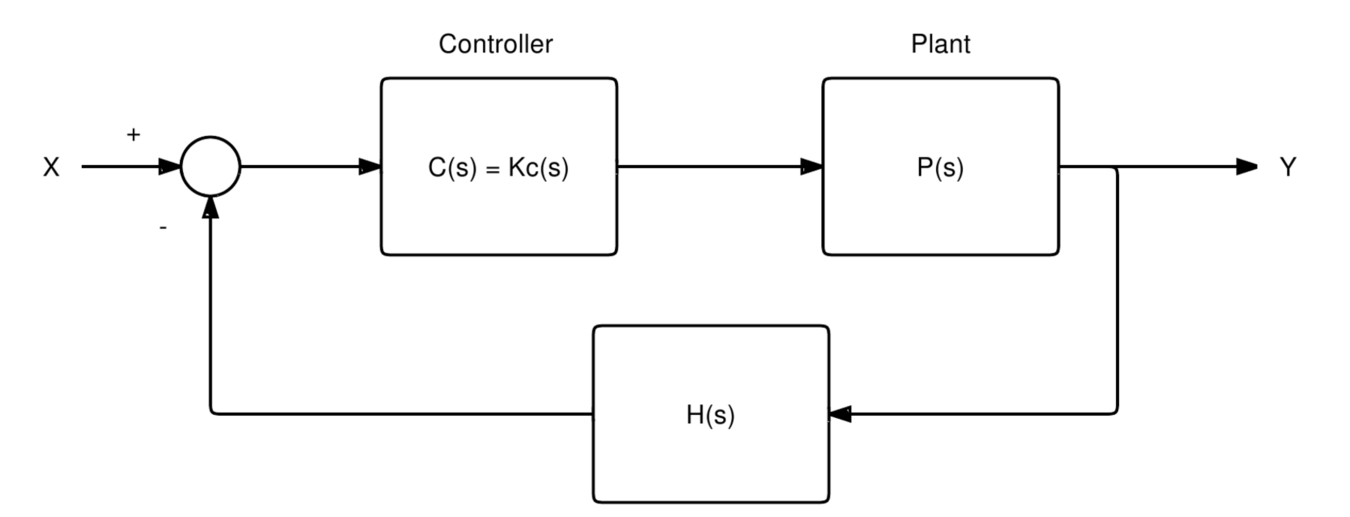
\includegraphics[width=4.5in]{figs11/cl_rl_systema.png}	%<sh>
\caption{A basic closed loop control system.}\label{basicCLfig}
\end{figure}

%
%
% \begin{itemize}
%  	\item  $P(s)$ is the ``Plant" -- expensive to change dynamics
% 	\item  $C(s)$ is the ``Controller" or ``Compensator" --- cheap to change (software).  In the diagram, we have broken it down to a constant real gain, $K$, and the rest of the transfer function, $c(s)$ such that $C(s)=Kc(s)$.
% \end{itemize}

%\end{frame}  %%%%%%%%%%%%%%%%%%%%%%%%%%%%%%%%%%%%%%%%%%%%%%%%%%%%%%%%%%%%

%%%%** Section 2
\section{System Type and Steady State Error}

In this section, we will examine the ``error" we have computed in control systems at the summing junction on the left side of the closed loop negative feedback system (Figure \ref{basicCLfig}).  Since in control systems, we most often consider $H(s) = 1$,  the error ($E(s) = X(s)-H(s)Y(s)$)
is a direct comparison between the input and the output.  In some applications, (consider a medical device or a flight control system for an interplanetary spacecraft) it is critical to eliminate error.  In others (consider a temperature control system for buildings) an error of one or two percent might not matter.

``Steady State" refers to the error between input and output as $t\to\infty$.  In practical applications, 
what do we mean by infinite time?  
We really mean the time that all transient terms become of insignificant magnitude.   For example, if 
\[
y_1(t) = 5e^{-0.1t}
\]
then for $t = 85$sec, $y_1(85) = 0.001$; a very small value compared to the amplitude 5.  For $t=85$, 
the transient due to $y_1(t)$ is ``over". On the other hand, for 
\[
y_2(t) = 5e^{-20t}
\]
then for $t = 0.425$sec, $y_2(0.425) = 0.001$.   For $y_2(t)$,  0.43 sec is essentially infinite.   
Thus ``infinite" time depends on the real part of the system's closed loop poles. 

It turns out that a key variable in studying the magnitude of error in a closed loop negative feedback system 
is the number of poles at the origin in the loop gain ($C(s)P(s)H(s)$ of Figure \ref{basicCLfig}). We 
call this number the {\it system type}.  The error also critically depends on the kind of input.  Some 
inputs are simply easier to track than  others.

\noindent
Some key points about system type and steady state error:
 \begin{itemize}
 	\item System {\bf ``type"} is \# of poles at origin: $\frac{1}{s^n}$ in the controller/plant

 	\item Input of amplitude $A$ can be
 	$
 	\left \{
  	\begin{array}{lc}
 	\mathrm{Step}		&    \frac{A}{s}   \\
 	\mathrm{Ramp}		&    \frac{A}{s^2}  \\
 	\mathrm{Parabola}	&    \frac{A}{s^3}  \\
 	\end{array}
 	\right .
        $

 	\item  If input is $\frac{A}{s^n}$, and your controller has {\it at least} $n$ type,
 		then there will be zero steady state error.
 \end{itemize}


%%%%** Example 1
\begin{ExampleSmall}
Find the system type for a closed loop negative feedback system consisting of the following elements:


 \[
 C(s) = \frac{500}{s(s+10)} \qquad P(s) = \frac{(s+0.1)}{s(s^2+50s+1500)} \qquad H(s) = 1
 \]

 \vspace{0.25in}
Every factor in the denominatory of $s$ by itself (i.e. $(s+0)$ ) is a pole at the origin. 
The combined system $CPH(s)$ has {\bf two} poles at the origin ($s^2$) so it is of {\bf type 2}.
\end{ExampleSmall}







%\end{frame}  %%%%%%%%%%%%%%%%%%%%%%%%%%%%%%%%%%%%%%%%%%%%%%%%%%%%%%%%%%%%

%%%%** Section 2.1
\subsection{Steady State Error Derivation}

The key to computation of steady state error is the Final Value Theorem of basic Laplace Transform theory:

\bq\label{FVTheorem}
\lim_{t\to\infty} f(t) = \lim_{s\to 0} sF(s)
\eq
Applying this to the system error $E(s)$, 
\bq
\lim_{t\to\infty} e(t) = \lim_{s\to 0} sE(s)
\eq
The quantity on the left is the steady state error, after all transient terms have died out.   The Final Value Theorem says we can find this final SSE by evaluating the limit on the right.  However, this theorem only applies if the limit on the left actually exists.  For example, if
$e(t) = B\sin(\omega t)$, then the limit does not exist.  Looked at in the complex plane, the poles of $E(s)$ must be in the left half plane so that all transients die out.

Now let's apply the FVT to the expression for error.
\[
E(s) = X(s) - C(s)P(s)H(s)E(s)
\]
abbreviating $G(s) = C(s)P(s)$, and simplifying,
\[
E(s) \left( 1+GH \right) = X(s)
\]

\bq\label{ErrorResult}
E(s) = \frac {X(s)} {1+GH}
\eq

Let's apply this result to a specific system where:
\[
C = 10 \qquad P = \frac{50}{s+10} \qquad H = 1 \qquad X(s) = \frac{A}{s}
\]
Note that we have chosen a specific input (step function with amplitude $A$), for this analysis.

Using Equation \ref{ErrorResult},
\[
E(s) = \frac{A/s}{(1+500/(s+10))} = \frac{A(s+10)}{s(s+10+500)}= \frac{A(s+10)}{s^2+510s}
\]
Applying the FVT:
\[
\lim_{t\to\infty} e(t) = \lim_{s\to 0} s\;\frac{A(s+10)}{s^2+510s} = \lim_{s\to 0} \frac{A(s+10)}{s+510} = \frac{10A}{510}
\]

\[
\lim_{t\to\infty} e(t) =  0.02A
\]
In other words the Steady State Error (SSE) is 2\%.


%%%%** Section 2.2
\subsection{Steady State Error Examples}

The following examples illustrate some key properties of steady state error.

%%%%** Example 2
\begin{ExampleSmall}
\[
C = 10 \qquad P = \frac{50}{s+10} \qquad H = 1 \qquad x(t) = Bt \qquad X(s) = \frac{B}{s^2}
\]
This is the same as above, but the input is now a ramp.

\[
E(s) = \frac{B/s^2}{1+\frac{500}{(s+10)}} = \frac{B(s+10)}{s^2(s+10+500)}= \frac{B(s+10)}{s^3+510s^2}
\]
Applying the FVT:
\[
\lim_{t\to\infty} e(t) = \lim_{s\to 0} s\;\frac{B(s+10)}{s^3+510s^2} = \lim_{s\to 0} \frac{B(s+10)}{s^2+510s} = \infty
\]
The system is the same, but with a ramp input the steady state error is infinite!

\end{ExampleSmall}



%%%%** Example 3
\begin{ExampleSmall}\label{ExIntwRamp}

\[
C = \frac{10}{s} \qquad P = \frac{50}{s+10} \qquad H = 1 \qquad x(t) = Au(t) \qquad X(s) = \frac{A}{s}
\]
This is the same as the first example, but the controller, $C(s)$, now adds a pole at the origin.
 \[
E(s) = \frac{A/s}{(1+\frac{500}{s(s+10)})} = \frac{A(s^2+10s)}{s(s^2+10s+500)}
\]
Applying the FVT:
\[
\lim_{t\to\infty} e(t) = \lim_{s\to 0} \frac{A(s^2+10s)}{s^2+10s+500} = 0
\]

The plant was the same, but by adding a pole at the  origin to the controller, we have eliminated SSE for step input to zero.
Since this is such a nice result it is worth a look at this new controller (Figure \ref{SimpleIntegralController}).
This controller can be implemented by building an integrator.  Two ways to implement an integrator are an analog op-amp circuit with a feedback capacitor, 
or alternatively, a software loop in a microcontroller which sums the difference between input and output.

\end{ExampleSmall}


%%%%** Figure 2
\begin{figure}\centering
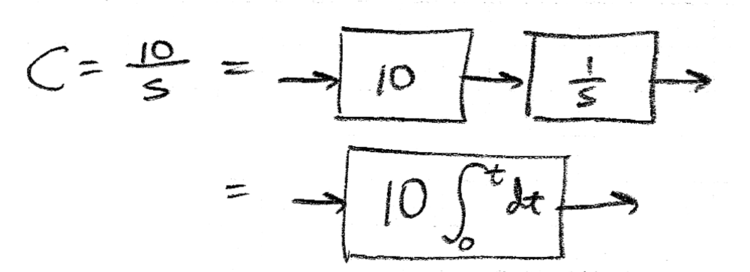
\includegraphics[width=2.5in]{figs09/00786a.png}
\caption{A simple controller which has a single pole at the origin can be called an {\it Integral controller}}\label{SimpleIntegralController}
\end{figure}





%%%%** Example 4
\begin{ExampleSmall}\label{ExIntegwithRamp}
\[
C = \frac{10}{s} \qquad P = \frac{50}{s+10} \qquad H = 1 \qquad x(t) = Bt \qquad X(s) = \frac{B}{s^2}
\]
This is the same as Example \thechapter.\ref{ExIntwRamp}, but the input is now a ramp.

\[
E(s) = \frac{Bs(s+10)}{s^2(s^2+10s+500)}
\]
Applying the FVT:
\[
\mathrm{SSE} = \lim_{s\to 0} \frac{sBs(s+10)}{s^2(s^2+10s+500)} = \lim_{s\to 0} \frac{B(s+10)}{s^2+10s+500}
\]
\[
= \frac{10}{500}B = 0.02B
\]
With the new controller, we have changed the SSE for ramp input from $\infty$ to 2\%!   Our controller has increased the system type by one and this made a big difference on SSE with the ramp input.

Note that calling the error ``2\%" is somewhat unclear for a ramp input.  Since B is a constant, but the input signal is $x(t) = Bt$, the error is a smaller and smaller percentage of the total input as time goes on.  In the steady state this error is finite but $0\%$!.

\end{ExampleSmall}



%%%%** Section 2.3
\subsection{Steady State Error Summary}

We've seen examples of how changing the system type or changing the input can make a big difference in the amount of steady state error.  You might even notice a pattern in the examples above relating the ``input type" (the power of $s$ in the Laplace transform of the input signal) and the system type to the nature of the SSE.  To see this relationship, let's take a closer look at Example \thechapter.\ref{ExIntegwithRamp}.

Writing out the limit again without canceling any terms,
\[
\mathrm{SSE} = \lim_{s\to 0} \frac{sBs(s+10)}{s^2(s(s+10)+500)}
\]
We have two $s$'s on the top.  One comes from the final value theorem, and the second one from the denominator of $C(s)$.  On the bottom, we have $s^2$, which comes from the ramp input.    The FVT term and the $C(s)$ denominator term combine to cancel the $s^2$ from the ramp input.   Thus, if the input is
\[
X(s) = \frac{A}{s^n}
\]
then we need at least $n-1$ poles at the origin in the combined controller and plant (again assuming $H=1$).


%%%%** Example 5
\begin{ExampleSmall}
Now we'll consider a general system with a gain factor, $K$, and $n$ poles at the origin in the controller, as well as a general input (i.e. $X(t) = Bt^m$) where $m=1$ means a ramp input, $m=2$ means a parabolic input, etc.
\[
C = \frac{K}{s^n} \qquad P = \frac{50}{s+10} \qquad H = 1 \qquad x(t) = Bt^m \qquad X(s) = \frac{B}{s^m}
\]

\[
\mathrm{SSE} = \lim_{s\to 0} \frac{s}{s^m} \frac{B}{\left(1+\frac{K}{s^n}\frac{50}{(s+10)}\right) }
\]

\[
\lim_{s\to 0} \frac{1}{s^{m-1}} \frac {Bs^n(s+10)} {(s^n(s+10)+50K)} = \lim_{s\to 0} \frac{Bs^n(s+10)} {s^{n+m}+10s^{n+m-1} + 50Ks^{m-1}}
\]


For this limit to be finite as $s\to 0$, we need to have no remaining powers of $s$ in the denominator after cancelation.  Thus  if
\[
n > m-1
\]
the error if zero.   If $n=m-1$ we have after cancellation
\[
\mathrm{SSE} = \lim_{s\to 0} \frac  {Bs^n(s+10)}   {s^{2n-1} + 10s^{2n-2} + 50Ks^n} = \frac {10B}  {50K}
\]
\end{ExampleSmall}



All of the relationships illustrated by these examples can be summed up in Table \ref{SystemTypeError}.
It is worth remembering that SSE only applies after transients (due to the non-zero poles) are over.  Such transients are illustrated for some typical situations in Figure \ref{SSEtransients}


%%%%** Figure 3
\begin{figure}\centering
Input \hspace{0.75in}  System Type \hspace{0.5in} Response/SSE\\[0.1in]
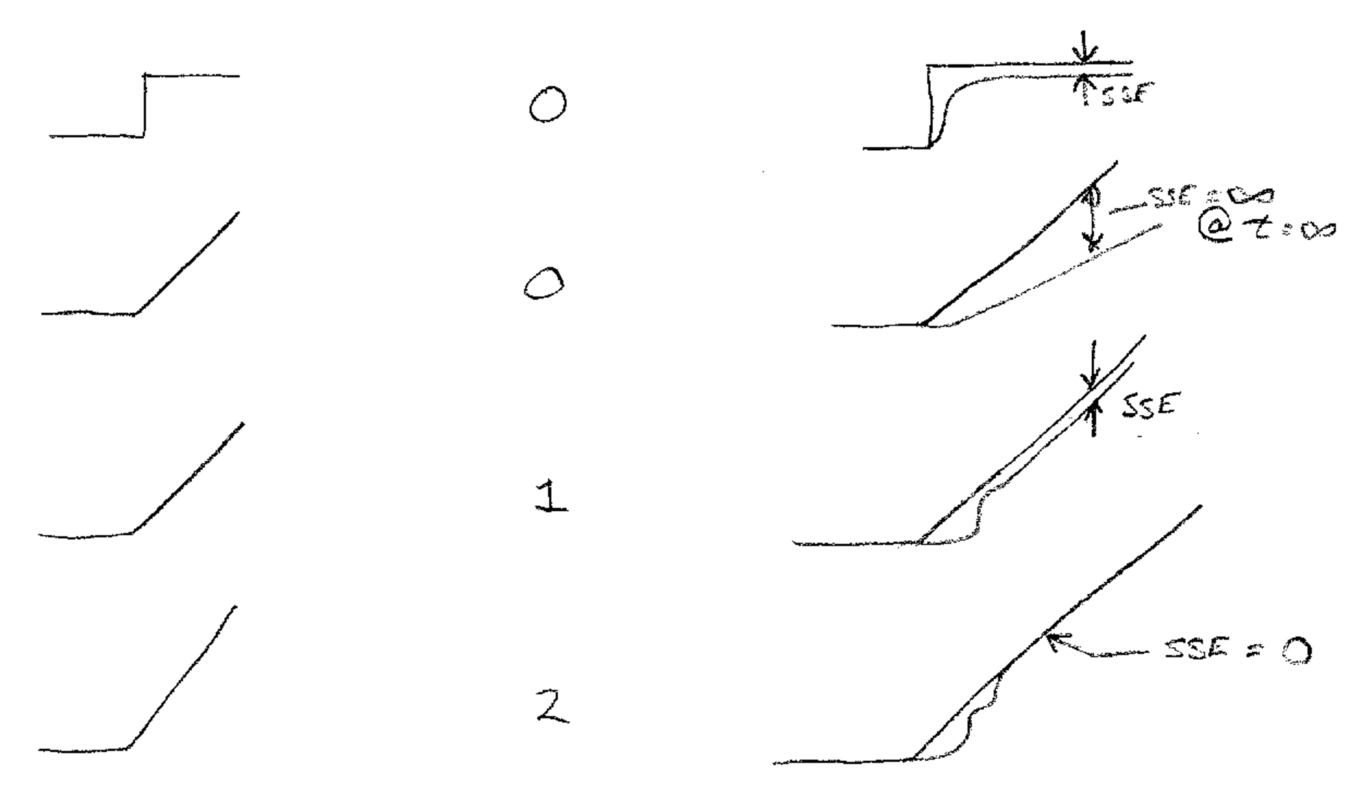
\includegraphics[width=4.50in]{figs11/00476a.png}\caption{Qualitative Illustrations of different SSE and transient responses.}\label{SSEtransients}
\end{figure}


%\end{frame}


%%%%** Table 1
\begin{table}\centering
\begin{tabular}{|c|c|c|c|c|} \hline
Type	&	$C(s)P(s)$	&	Step $(n=1)$	&	Ramp $(n=2)$	& 	Parabola $(n=3)$   \\ \hline
0	&	$K\dots$	&	finite		&	$\infty$	&	$\infty$	   \\ \hline
1	&	$\frac{K}{s}\dots$&	0		&	finite		&	$\infty$	   \\ \hline
2	&	$\frac{K}{s^2}\dots$&0		&       0        	&	finite		   \\ \hline
\end{tabular}

\caption{SSE vs. System Type and Input Type}\label{SystemTypeError}
\end{table}


%%%%%%%%%%%%%%%%%%%%%%%%%%%%%%%%%%%%%%%%%%%%%%%%%%%%%%%%%%%%%%%%%%%%%%%%%%%%%%%%%%%%%%%%%%%%%%%%%%%%%%%%%%%


%%%%** Section 3
\section{Time Domain Performance of 2nd Order Systems}

In this section we will describe some ways to measure the performance of system response.  While with steady state error we focused on the response after the transients died out, here we will focus on the transient characteristics of the step response in particular.

%%%%** Figure 4
\begin{figure}\centering
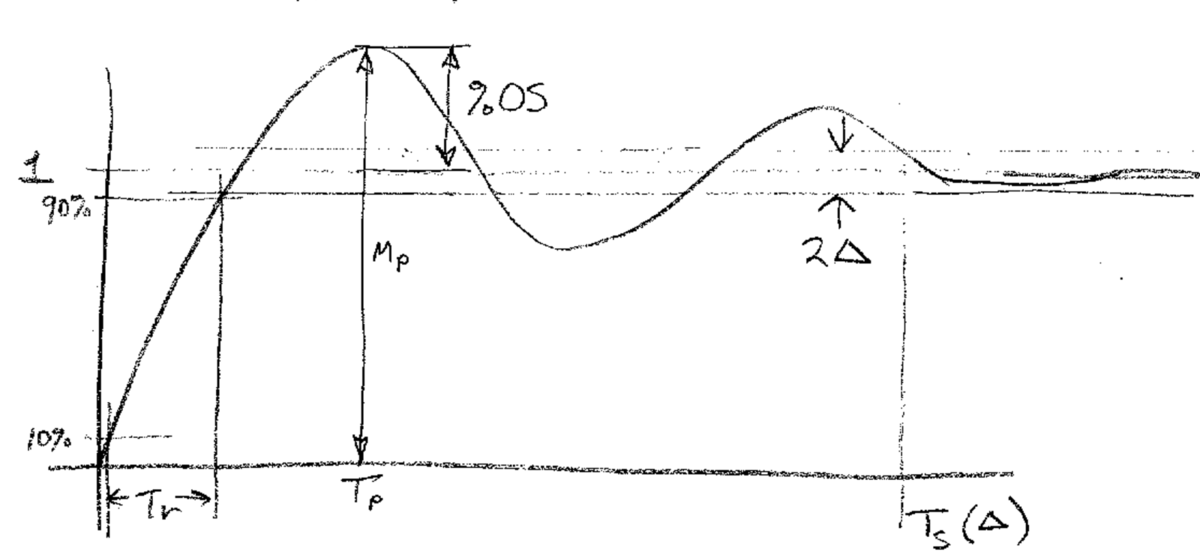
\includegraphics[width=4.0in]{figs11/00472a.png}
\caption{A step response with labels for percent overshoot (\%OS) and settling time, $T_S$.}\label{stepresponse}
\end{figure}


%%%%** Section 3.1
\subsection{Transient Performance Specifications}

The transient performance of second order systems (systems having 2 poles) is fairly easy to characterize.  We develop intuition about the relationship of pole locations to time response from these second order systems.  Although practical systems are usually higher order and we use computer techniques to fully understand their dynamics, the relationship between time domain performance and 2nd order poles is important to learn.

Looking at a typical step response (Figure \ref{stepresponse}), the most basic measures are 
\begin{enumerate}
    \item the time it takes to settle down
    \item the time it takes to reach close to the target
    \item the amount the response overshoots the target before it settles down.
\end{enumerate}

\subsubsection{Settling time, $T_s$}
If the input step has amplitude $A$,
{\it Settling time}, $T_s$ is defined as the time it takes for the transient to enter a window around the final value such that
\[
0.98A < y(t) < 1.02A   \qquad\quad \forall t > T_s
\]
In other words, $T_s$ is the {\it last} time $y(t)$ goes into a window of $\pm2\%$ around the final value.
We know that the sinusoidal component of the output response is bounded by the exponential envelope (Figure \ref{typicalstep}) and that the exponential envelope is
\[
\mathrm{env}(t) = e^{\sigma t}
\]
where $\sigma$ is the real part of the pole.  For the output response to be 2\% of the amplitude at $t=T_s$, we need
\[
e^{\sigma T_s} = 0.02
\]
In other words,

\[
T_s = \frac{\ln{0.02}}{\sigma} \approx \frac{-4}{\sigma}
\]

%%%%** Example 6
\begin{ExampleSmall}
Find the approximate settling time, $T_s$ for the following system:

\[
G(s) = \frac {10^7}  {(s+4.7+10j)(s+4.7-10j)}
\]

\vspace{0.25in}
The poles are $s=-4.7\pm10j$.  Therefore,
\[
T_s \approx \frac{-4}{-4.7}  = 0.85 \mathrm{sec}
\]
\end{ExampleSmall}



\subsubsection{Rise time, $T_r$}
{\it Rise Time}, $T_r$ is defined as the time taken by the step response to reach 90\% of the amplitude, $A$.  
There is no analytical expression for Rise time based on the pole locations.   However, for a range of damping ratios, $\zeta$,
we can determine the rise-time, expressed as a constant multiplied by the reciprocal of the systems natural frequency $\omega_n$:
\begin{equation}
T_r = \frac{1}{\omega_n}F(\zeta)
\end{equation}
where $F()$ is an empirical function measured by numerical simulations (Table \ref{percentOStable}).   Two curves fit to this function are
\begin{equation}
T_r \approx \frac{1}{\omega_n}(1.76\zeta + 0.824) \qquad   0.1< \zeta < 0.8
\end{equation}
and

\begin{equation}\label{Tr_non_lin}
T_r \approx \frac{1}{\omega_n}(2.23\zeta^2 - 0.78\zeta + 1.12)
\end{equation}
We can use the non-linear equation (eqn \ref{Tr_non_lin}) if more accuracy is required.
In practice however, settling time, $T_s$ is a more practical specification for use in design and $T_r$ is less often used. 


\subsubsection{Overshoot, \%OS}

Overshoot is expressed as a percentage of the input amplitude.   In some applications a brief tansient overshoot is acceptable.  In other applications, (think of a elevator controller) overshoot is unacceptable\footnote{There are other techniques called Trajectory Generators, beyond the scope of this chapter, which can be used to eliminate overshoot.}.

The analytical calculation of overshoot from second order systems is somewhat involved.  A few computational results gives a lookup table (Table \ref{percentOStable}) in which overshoot depends on the damping ratio, $\zeta$ (Chapter \ref{2ndOrderTransientChapter}), or 
equivalently the angle formed by the complex conjugate poles ($\theta = \cos^{-1}(\zeta)$.)

%%%%** Table 2
\begin{table}[h]\centering
\begin{tabular}{c|c|c|c}
	\%OS	& $\zeta$	& $T_r$          &   $\theta$	\\\hline
	10\%	& 0.587		& $1.8/\omega_n$ &  54$^\circ$	\\
	 5\%	& 0.695		& $2.1/\omega_n$ &  46$^\circ$	\\
	 2\%	& 0.777		& $2.3/\omega_n$ &  39$^\circ$	\\
	 1\%	& 0.829		& $2.6/\omega_n$ &  34$^\circ$	\\
\end{tabular}
\caption{Table of numerically computed values of percent overshoot vs. damping ratio ($\zeta)$.    $T_r$ is also shown for
completeness. Note that rise time gets longer as overshoot is reduced.}\label{percentOStable}
\end{table}

%%%%** Section 3.2
\subsection{S-plane Regions}

The performance specifications, $T_s$ and \%OS,  correspond to constraints on where the poles can be located.
Since  $T_s = -4/\sigma$, requiring a  specification for $T_s$ requires that the poles lie somewhere along a vertical line at $\sigma = -4/T_s$ (recall that $\sigma$ is the real part of the poles).  Similarly, using  Table \ref{percentOStable}, we can see that an exact overshoot specification requires that the poles lie on a line from the origin at the angle determined by the lookup table.


%%%%** Example 7
\begin{ExampleSmall}
A 2nd order system has the following transient step response specifications.
\[
T_s = 0.01 \mathrm{sec} \qquad \%OS = 5\%
\]

Find where the poles must be located.

\vspace{0.1in}
----

We know the real part of the poles  must be
\[
\sigma = -4/0.01 = -400
\]
but at the same time, based on Table \ref{percentOStable}, the angle the pole makes with the negative real axis must be $46^\circ$.  The only point which meets both specs is the intersection of these two lines.

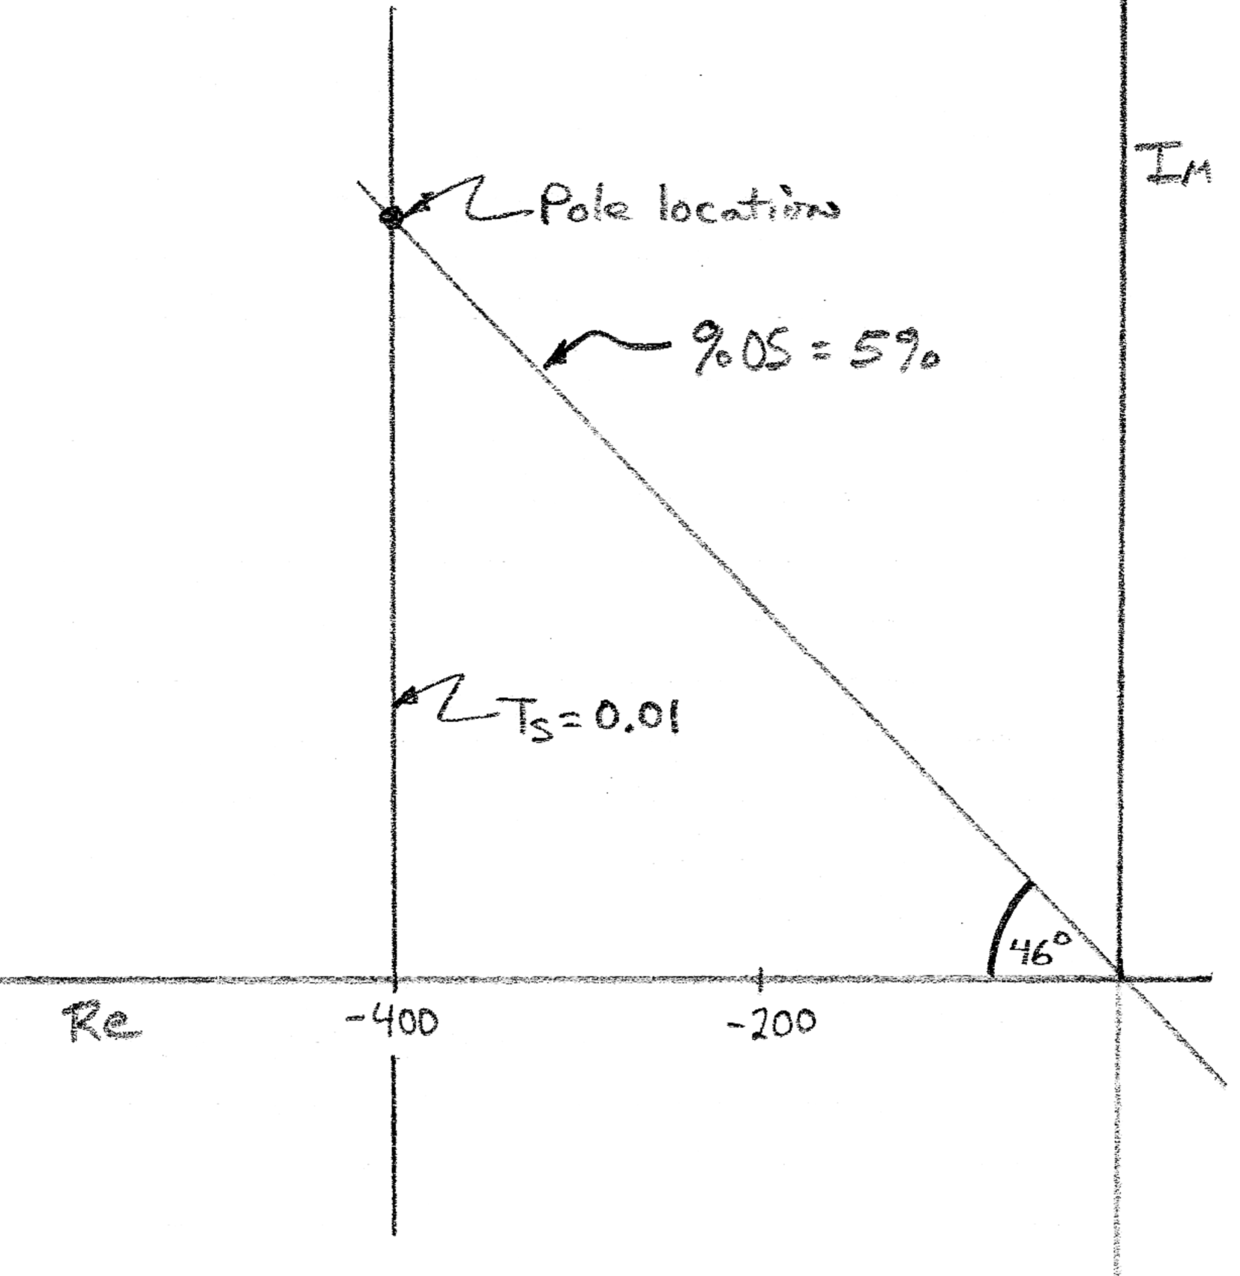
\includegraphics[width=105mm]{figs09/00787a.png}

\end{ExampleSmall}



Sometimes specifications are expressed in terms of inequalities.  For example, if the specification is $T_s \leq 0.25$, then any pole location to the left of $\sigma  = -0.25$ meets the specification.  In drawing inequality performance specs in the $s$ plane, we shade the region which the poles should NOT occupy to meet the spec.   Two inequality specifications generate a region in the $s$-plane which the poles must be in to meet the specifications (Figure \ref{splaneregion}).


%%%%** Figure 5
\begin{figure}\centering
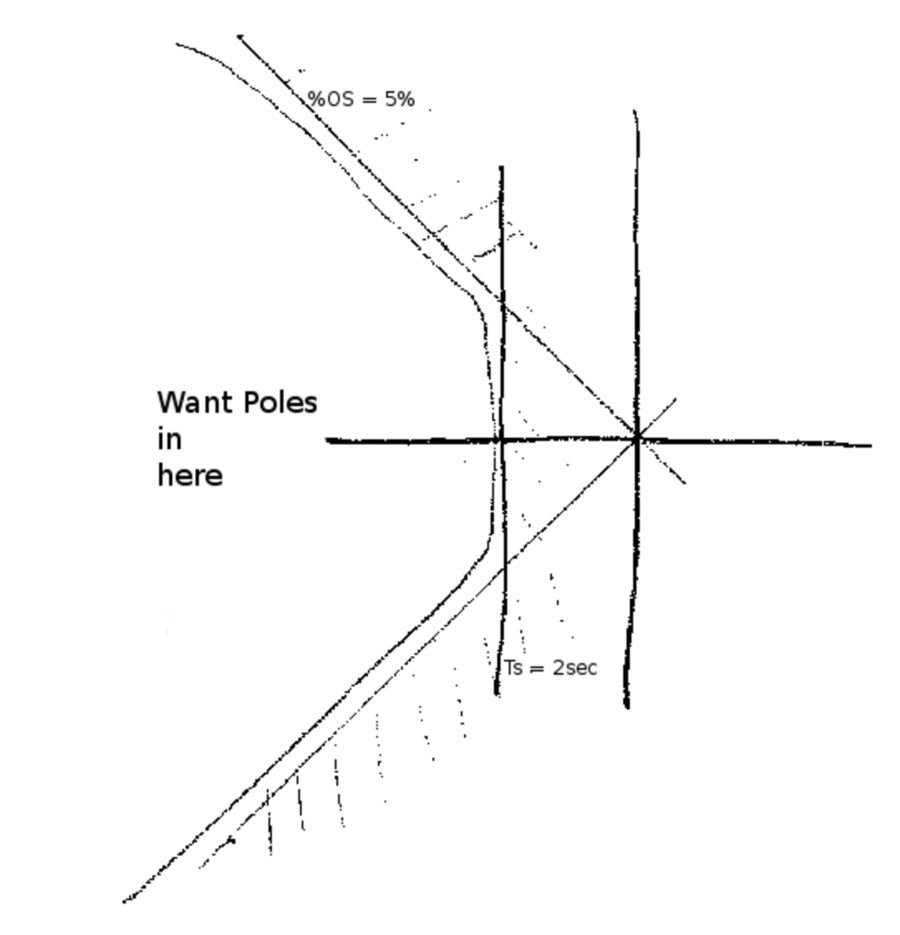
\includegraphics[width=3.0in]{figs11/00473a.png}
\caption{Any poles in the non-shaded region will meet  the specs: $\%OS \leq 5\%$ and $T_S \leq 2ms$.}\label{splaneregion}
\end{figure}

%%%%** Section 3.3
\subsection{S-plane Performance Region Examples}


%%%%** Example 8
\begin{ExampleSmall}
Find the $s$-plane region in which poles of a 2nd order system meet the following specifications:
\[
T_s < 10 \mathrm{sec} \qquad \%OS < 1\%
\]

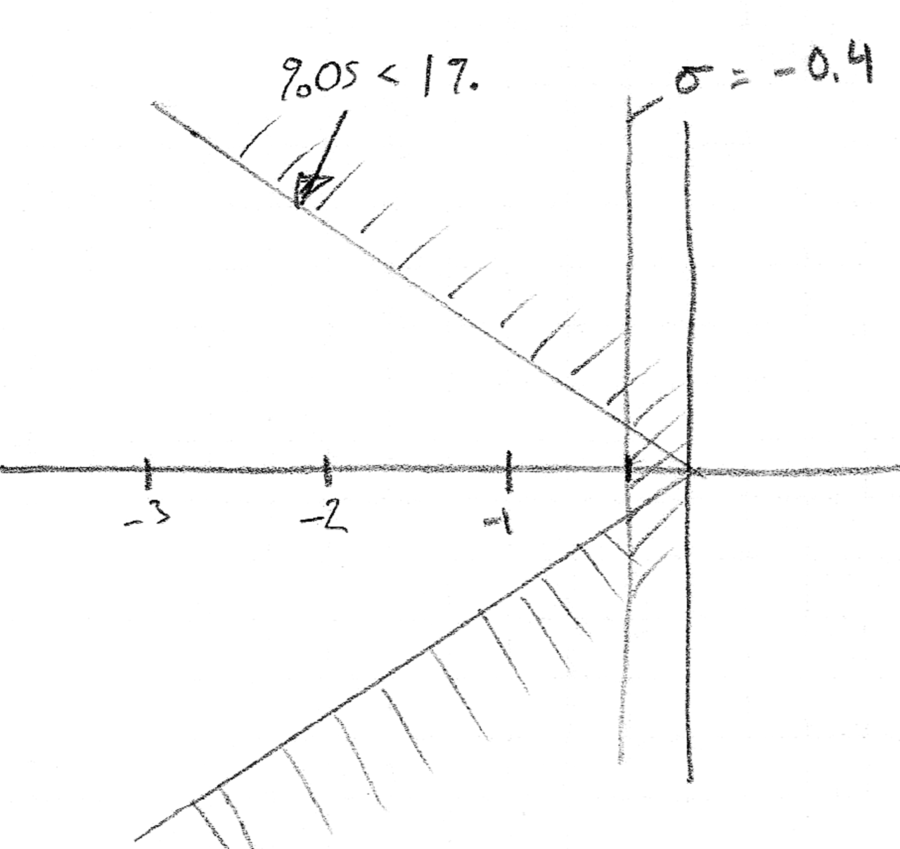
\includegraphics[width=3.in]{figs09/00788a.png}

Since these are inequality specs, we shade the regions above the diagonal ($\%OS$) and to the right of the vertical ($T_S$).  Poles must be in the {\it non-shaded} region to meet the specs.
\end{ExampleSmall}


%%%%** Example 9
\begin{ExampleSmall}
Find the $s$-plane region in which poles of a 2nd order system meet the following specifications:
\[
T_s < 0.2 \mathrm{sec} \qquad \%OS < 10\%
\]
As in the previous example, shade the region that {\bf DOES NOT} meet the specs. 

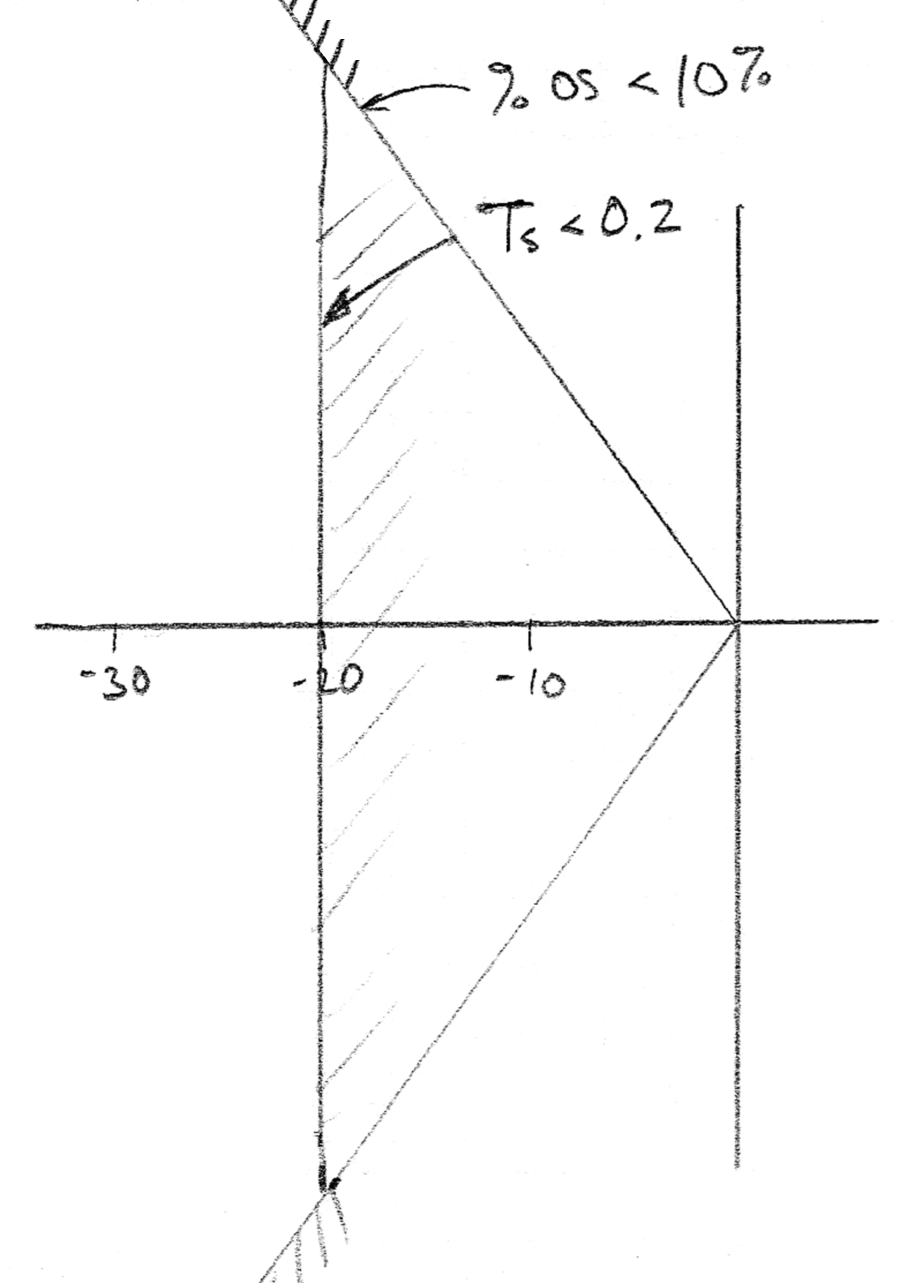
\includegraphics[width=2.5in]{figs09/00789a.png}
\end{ExampleSmall}

%%%%** Example 10
\begin{ExampleSmall}
Find the $s$-plane region in which poles of a 2nd order system meet the following specifications:
\[
T_s < 1 \mathrm{sec} \qquad 2\% < \%OS < 10\%
\]

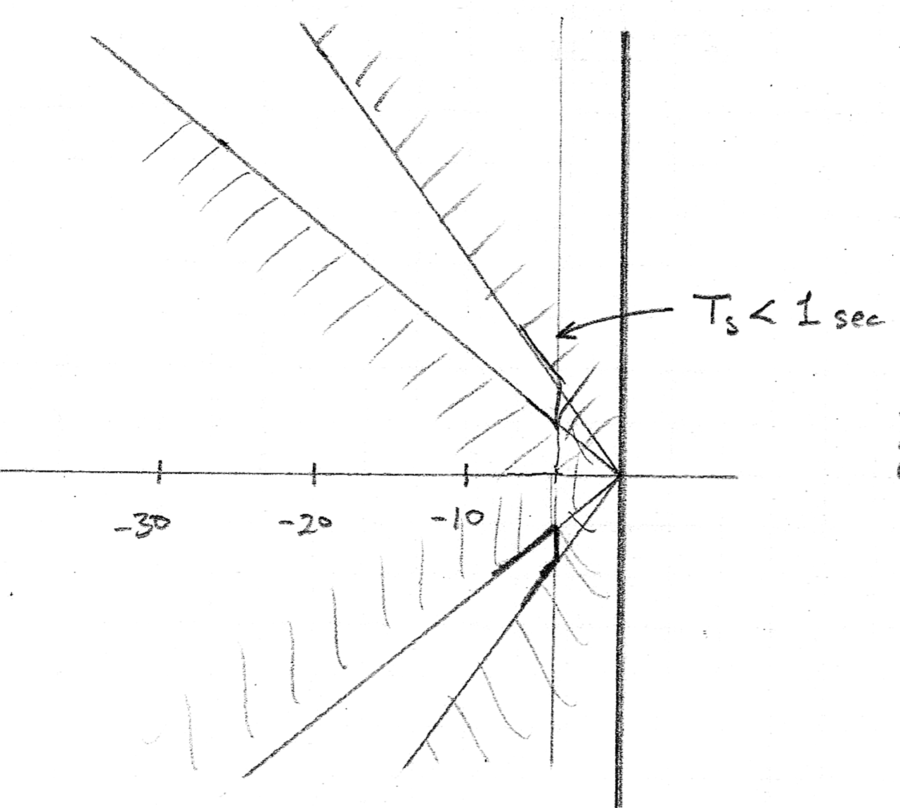
\includegraphics[width=2.5in]{figs09/00790a.png}
\end{ExampleSmall}

%%%%** Example 11
\begin{ExampleSmall}
Find the $s$-plane region in which poles of a 2nd order system meet the following specifications:
\[
0.5 < T_s < 2.0 \mathrm{sec} \qquad \%OS = 5\%
\]

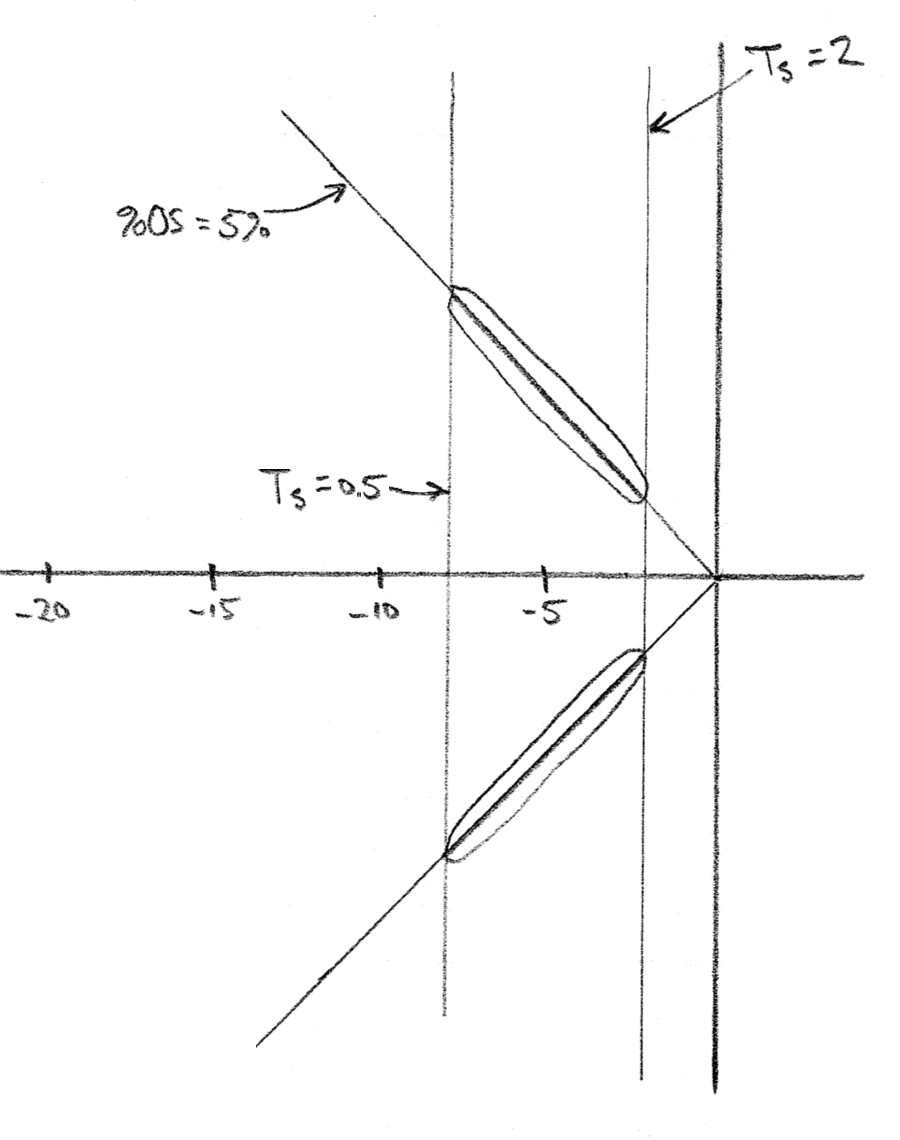
\includegraphics[width=3.in]{figs09/00791a.png}

Note that since the $\%OS$ spec is an equality, the ``region" is actually a line segment. 

\end{ExampleSmall}





%%%%%%%%%%%%%%%%%%%%%%%%%%%%%%%%%%%%%%%%%%%%%%%%%%%%%%%%%%%%%%%%%%%%%%%%%%%%%%%%%%%%%%%%%%%%%%%%%%%     Control Effort

%%%%** Section 4.5
\section{Control Effort}\label{CtlEff}

%\begin{frame}
%\frametitle{Control Effort}

Control effort is the level of output needed by the controller to achieve the step response.  
All other things being equal, a controller which achieves the specs with lower control effort is better.  
Often there is a limited maximum effort that a given system can output.  
For example, a DC motor has a maximum torque that it is capable of (without overheating). 
In this case, it is meaningless to have 
a settling time that is very fast if that requires 10 times more torque that the motor's maximum limit.  
For some plants, controller gains can be found to meet {\bf any} $T_S$ and $\%OS$ spec if control 
effort limits are ignored. 

Computing control effort is easy.  Consider the system of Figure \ref{controleffort}  which has a controller, plant and feedback.	%<h>

%\end{frame}  %%%%%%%%%%%%%%%%%%%%%%%%%%%%%%%%%%%%%%%%%%%%%%%%%%%%


%\begin{frame}



%%%%** Figure 8
\begin{figure}\centering
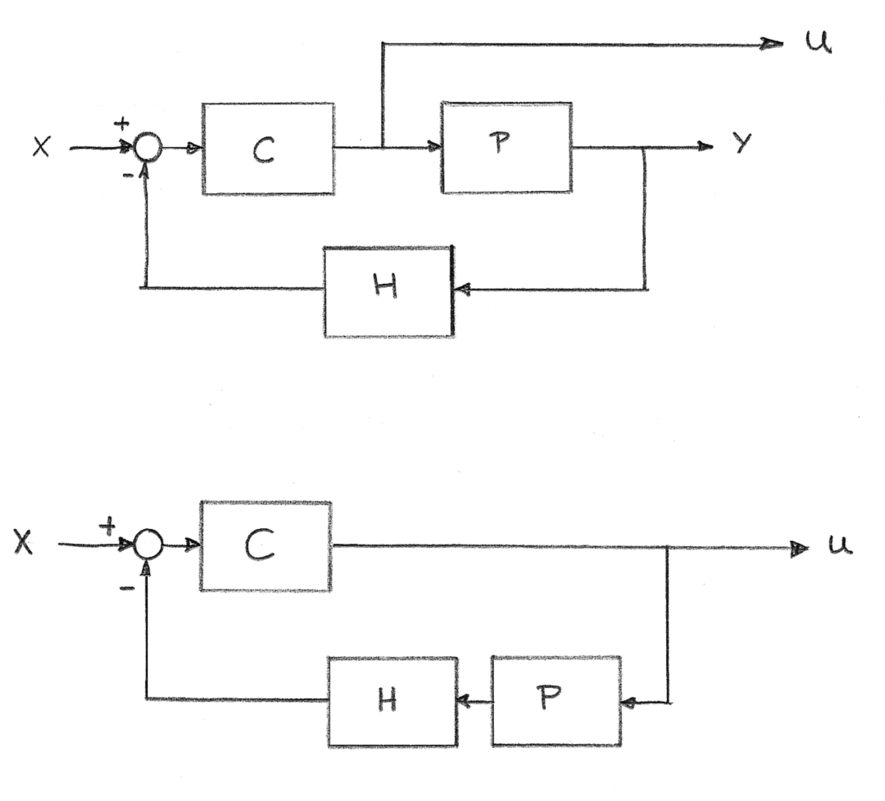
\includegraphics[width=75mm]{figs11/00650a.png}
\caption{Control effort signal $u(t)$ or $U(s)$ comes from the output of the controller. We can easily get U by analyzing the bottom system.}\label{controleffort}
\end{figure}



%\end{frame}  %%%%%%%%%%%%%%%%%%%%%%%%%%%%%%%%%%%%%%%%%%%%%%%%%%%%



%\begin{frame}
The top system looks conventional, except we have brought out the control effort signal.   In the second system we have simply rearranged the blocks without changing any connections.   However we can now see this as a new feedback system having feedforward path $C$ and feedback $PH$.  Giving the traditional name  $U$ to the control output,	%<h>
\[
\frac{U(s)}{X(s)} = \frac {C(s)}  {1+C(s)P(s)H(s)}
\]

%\end{frame}  %%%%%%%%%%%%%%%%%%%%%%%%%%%%%%%%%%%%%%%%%%%%%%%%%%%%


%\begin{frame}
%\frametitle{Control Effort Metrics}
If we have a limit on our actuator, for example,	%<h>
\[
\tau_{max} = 1.5 NM
\]
then an appropriate measure of performance would be the maximum value of $u(t)$: does it exceed 1.5$NM$? .   On the other hand, if we are concerned with total energy consumption, an appropriate measure might be	%<h>
\[
\int_0^{Tmax} u^2(t) dt
\]
where $T_{max}$ defines a time window that makes sense for our application.	%<h>

\begin{Example}
Compute the control effort for step input for the system consisting of controller, $C(s)$ and plant, $P(s)$:
\[
C(s) = \frac  {k(s+2)}  {s(s+20)}  \qquad P(s) = \frac   {0.5}  {(s+0.5)} \qquad H(s) = 1
\]
for three gains:
\[
k = [0.5, 5, 100]
\]
Using scilab we will plot the closed loop system step response for the input $X(s) = 1/s$ (the unit step):
\[
Y(s) = X(s) \frac  {C(s)P(s)}  {1+C(s)P(s)}
\]
and control effort:
\[
U(s) = X(s)\frac {C(s)}  {1+C(s)P(s)}
\]

\begin{centering}
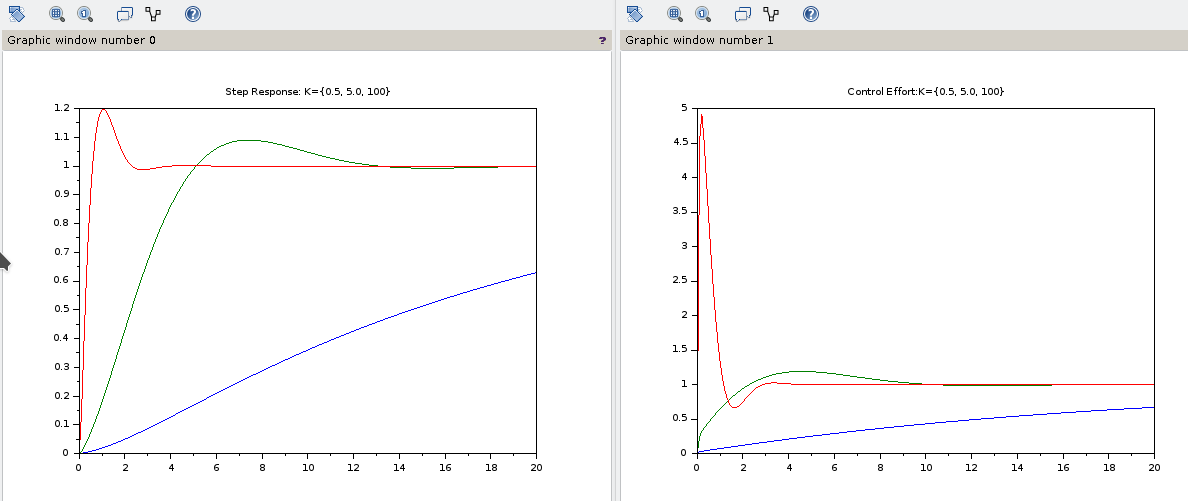
\includegraphics[width=6.25in]{figs09/step_ctl_effort_scilab.png}
\end{centering}

The responses are colored as follows: 
\begin{tabular}{r|r|r|r}
k     &  0.5 & 5   & 100 \\
\hline
color & blue & green & red \\
\end{tabular}

The highest gain (red) has a much faster response than the lowest gain (blue) but note how much higher is the 
control effort.   If for example, our maximum actuator capability is 1.5 units, we would have to limit our gain to 
something like $k=5$ (noting that the green line stays below that level), and expect correspondingly slower step response.
\end{Example}


%%%%%%%%%%%%%%%%%%%%%%%%%%%%%%%%%%%%%%%%%%%%%%%%%%%%%%%%%%%%%%%%%%%%%%%%%%%%%%%%%%%%%   PID Control


%%%%** Section 4
\section{PID Controller}
	%<*>
%%%%** Section 4.1
\subsection{Closed Loop Design Problem}

The design problem of closed loop controllers\footnote{Sometimes the controller is referred to as a ``compensator" but we will use ``controller".} can be summarized as follows (Assume 
for simplicity that $H=1$).  

\begin{quotation}   Given a plant: $P(s)$,  specify a controller, $C(s)$, for a closed loop system to improve some performance measure compared to the open loop system, $P(s)$.
Where the closed loop response is governed by   $\frac{C(s)P(s)}{1 + C(s)P(s)}$ 
\end{quotation}

%\end{frame}  %%%%%%%%%%%%%%%%%%%%%%%%%%%%%%%%%%%%%%%%%%%%%%


The Proportional-Integral-Derivative (PID) controller is a class of controllers which has
two zeros and one pole at the origin.  The PID controller is the most common controller in industry BY FAR.   Design of the PID controller consists of deciding on the desired 
location of the two zeros and a single gain term, $K_D$.   

The PID controller an be expressed in three equivalent forms:
\bq
C(s) = \frac{K_Ps+K_Ds^2 + K_I}{s} = \frac{K_D(s^2 + \frac{K_P}{K_D}s+ \frac{K_I}{K_D})}{s} =
\frac{K_D(s+z_1)(s+z_2)}{s}
\eq
All three depend on three positive real gains for the engineer to design: $K_P, K_I, K_D$.
Lower order forms of the PID
controller with one or no zeros are also possible according to the values of the three gains.
The response of the closed loop system depends only indirectly on the zeros and pole of the 
PID controller because the  closed loop system has a root locus and its response depends on 
were we are.   However the zeros of the PID controller can ``pull" the closed loop root-locus 
pole pathways, usually towards the left, which drives faster response and greater stability. 
The PID controller's pole at the origin can increase the system type and thus reduce 
steady state error. 

 
%%%%** Figure 6
\begin{figure}\centering
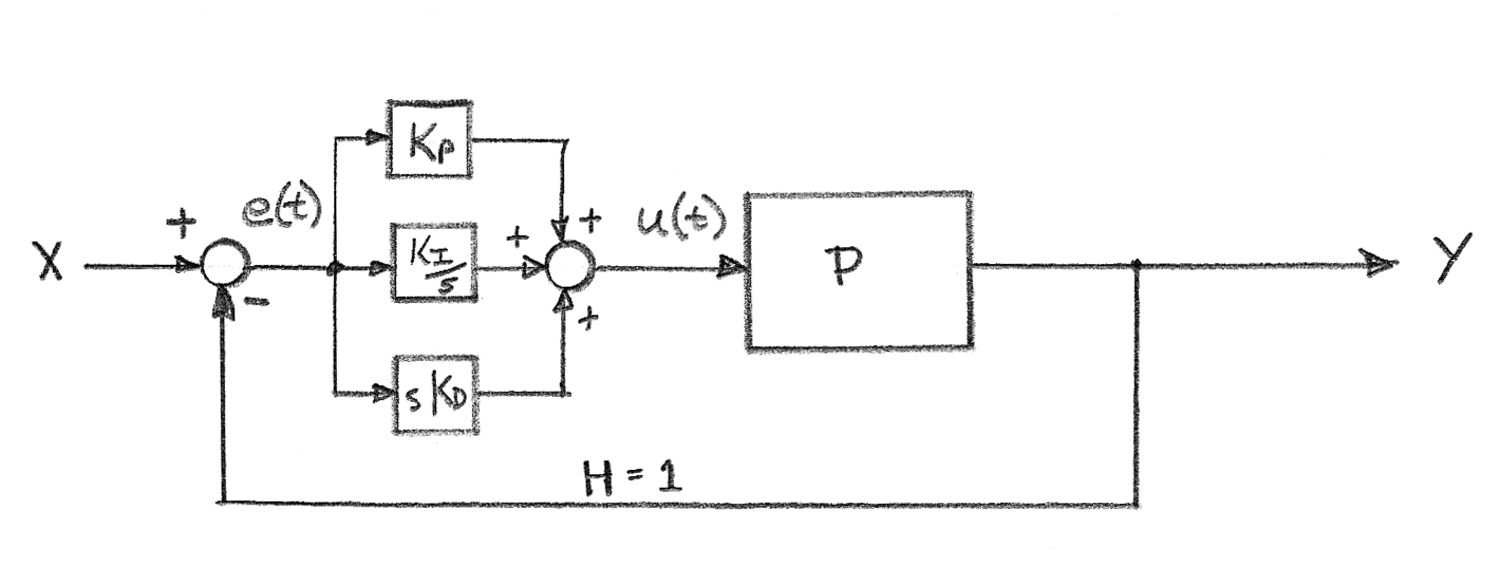
\includegraphics[width=5.0in]{figs11/00651a.png}
\caption{The PID controller.}\label{PIDBlockDiagram}
\end{figure} 


%%%%** Section 4.3
\subsection{Basics}

%\begin{frame}
%\frametitle{Basics}

The PID controller and a  plant (P) are illustrated in Figure \ref{PIDBlockDiagram}. Interpreting the block diagram,

\begin{equation}\label{PID}
C_{PID}(s) = \frac{U(s)}{E(s)} = K_P + \frac{K_I}{s} + K_Ds
\end{equation}
and equivalently
\begin{equation}\label{PID2}
C_{PID}(s) =  \frac{K_Ps+K_i + K_Ds^2}{s} = \frac{K_D(s^2 + \frac{K_P}{K_D}s + \frac{K_I}{K_D})}{s}
\end{equation}

%\end{frame} %%%%%%%%%%%%%%%%%%%%%%%%%%%%%%%%%%%%%%%%%%%%%%%%%%%%%%



%\begin{frame}
{\bf $K_P$}  is the proportional gain.
Looking at the first term of Equation \ref{PID}, you can see that $K_P$ directly multiplies the error (the input to the controller).  If the other gains were zero, the control output, $u$, will be  linearly proportional to error.	%<h>

\[
u(t) = K_P e(t)
\]

%\end{frame} %%%%%%%%%%%%%%%%%%%%%%%%%%%%%%%%%%%%%%%%%%%%%%%%%%%%%%



%\begin{frame}
{\bf $K_I$} is the integral gain.
Looking at the second term of Equation \ref{PID2} we see that $K_I$ appears multiplied by $1/s$, the integral operator.  If the other gains were zero, the control output, $u$, would be $K_I$ times the time integral of the error:	%<h>

\[
u(t) = K_I \int_0^t e(t) dt
\]



%\end{frame} %%%%%%%%%%%%%%%%%%%%%%%%%%%%%%%%%%%%%%%%%%%%%%%%%%%%%%



%\begin{frame}
{\bf $K_D$} is the derivative gain.
Looking at the third term of Equation \ref{PID} we see that $K_D$ appears multiplied by $s$, the derivative operator.  If the other gains were zero, the control output, $u$, would be $K_D$ times the time derivative of the error:	%<h>

\[
u(t) = K_D \frac{d}{dt}e(t)
\]
In fact, using the inverse Laplace transform we can write:
\[
u(t) = K_P e(t)  + K_I \int_0^t e(t) dt + K_D \frac{d}{dt}e(t)
\]


Some alternate forms of the PID controller are given in of Equation \ref{PID2}.  These forms are useful as we design the PID controller for a specific system.
%\end{frame} %%%%%%%%%%%%%%%%%%%%%%%%%%%%%%%%%%%%%%%%%%%%%%%%%%%%%%



%%%%** Section 4.4
\subsection{Simulation of PID controllers}\label{simulationPIDcontrollers}

% 
% 
% %%%%** Figure 7
% \begin{figure}[h]\centering
% \includegraphics[width=2.50in]{figs09/pid_boxa.png}
% \caption{A Commercial PID Controller. (\$129, {\tt www.automationdirect.com})}\label{pidbox}
% \end{figure}


Looking again at equation (\ref{PID}), we can see from the far right hand side that the PID controller has two zeros and one pole.   A system with more zeros than poles cannot be physically realized and is called {\it improper}.   Often this condition is ignored because the plant has enough poles to make the overall forward path ($C(s)P(s)$) proper.  However, what if you would like to make and sell a PID controller box 
(search your favorite e-commerce site for "pid controller")?
% (Figure \ref{pidbox})?

We may also have this problem building a computer simulation if we define the controller in our script as a separate system and our simulation package (such as Scilab or Matlab)  cannot simulate an improper system.
To fix this we simply add another pole to the PID controller at a high enough frequency so that it does not affect our response.  This imediately raises two questions


%  Solution:  Add another high frequency pole:  $\frac{a}{(s+a)}$


\begin{enumerate}
  \item Why doesn't a high frequency pole affect the system?
  \item How high is ``high enough"?
\end{enumerate}

%\end{frame} %%%%%%%%%%%%%%%%%%%%%%%%%%%%%%%%%%%%%%%%%%%%%%%%%%%%%%%%%%%%%%%%%%




%\begin{frame}

For question one, consider the Bode plot of the basic one-pole system	%<h>

%\frametitle{Q1:  Why doesn't it effect the system?}

\[
P(s) = \rho/(s+\rho)
\]

for $\omega << \rho$, $P(j\omega) = 1$.  Its magnitude is 1 and its phase angle is 0.
Thus for frequencies substantially below $\rho$, $P(s)$ has no effect.	%<h>

%\end{frame} %%%%%%%%%%%%%%%%%%%%%%%%%%%%%%%%%%%%%%%%%%%%%%%%%%%%%%%%%%%%%%%%%%




%\begin{frame}
%\frametitle{Q2: How high is ``high enough"?}

For question two, let us set $\rho$ to be 10 times higher than the highest pole or zero of our system.   Technically we should know the zeros of the PID controller to do this, but if we {\it assume} that the zeros of a good controller will be in the neighborhood of the poles of the plant, then 10 times greater than the highest frequency plant pole/zero will also be far from the PID controller zeros.	%<h>

$\rho = 10\times pz_{max}$	%<sh>

where $pz_{max}$ is the highest pole or zero in the system.	%<h>

Thus we will add a pole, $\rho$,  to the PID controller in our simulations as follows:	%<h>

% \begin{equation}\label{PID2}
\[
C_{PID2}(s) = \frac{\rho(K_Ps+K_i + K_Ds^2)}{s(s+\rho)} = \frac{\rho K_D(s^2 + \frac{K_P}{K_D}s + \frac{K_I}{K_D})}{s(s+\rho)}
\]
% \end{equation}

Now $C_{PID2}$ is proper
because it has the same number of poles and zeros, two.  Thus, Scilab can simulate it and it is also physically realizable.	%<h>









%%%%** Section 5
\section{Manual Design of PID controller}\label{manualPIDdesign}
% \section{}

In this section we will design PID control gains through a ``manual" method.  Specifically we will find the values of $K_P, K_I, K_D$ for a given plant and a set of performance specifications, including control effort.  Although fully hand methods are discussed in standard textbooks, our ``manual" method uses the computer to speed Root Locus plotting and analysis.   With all but the simplest plants, hand methods are not accurate enough for real design.  Hand methods are still valuable to give a starting point for more accurate computer design methods discussed in the next chapter.

The computer optimization method of the next chapter will eventually find a great design (i.e. $K_P,K_I,K_D$ values), and can take more performance criteria into account, but it will go significantly faster with an initial starting guess.   Unfortunately there is no ``typical" range of PID parameter values which could be used as a standard starting range so to get the most utility from computer methods we should generate the rough initial design manually.


\begin{Example}
Let's get started with an example with really simple root loci:
\[
P(s) = \frac  {1}   {(s+1)(s+2)(s+10)}
\]
To keep things simple we will use two simplified PID controllers:   
\[
C_1(s) = K \qquad   C_2(s) = \frac   {K(s+0.1)} {s} 
\]
% To show that they are in fact PID: $\frac   {K(s+1)} {s}  =  \frac{Ks}{s} + \frac{K}{s} = 0s + K + K/s $, so 
% \[
% K_P=K, K_I = K, K_D=0
% \]

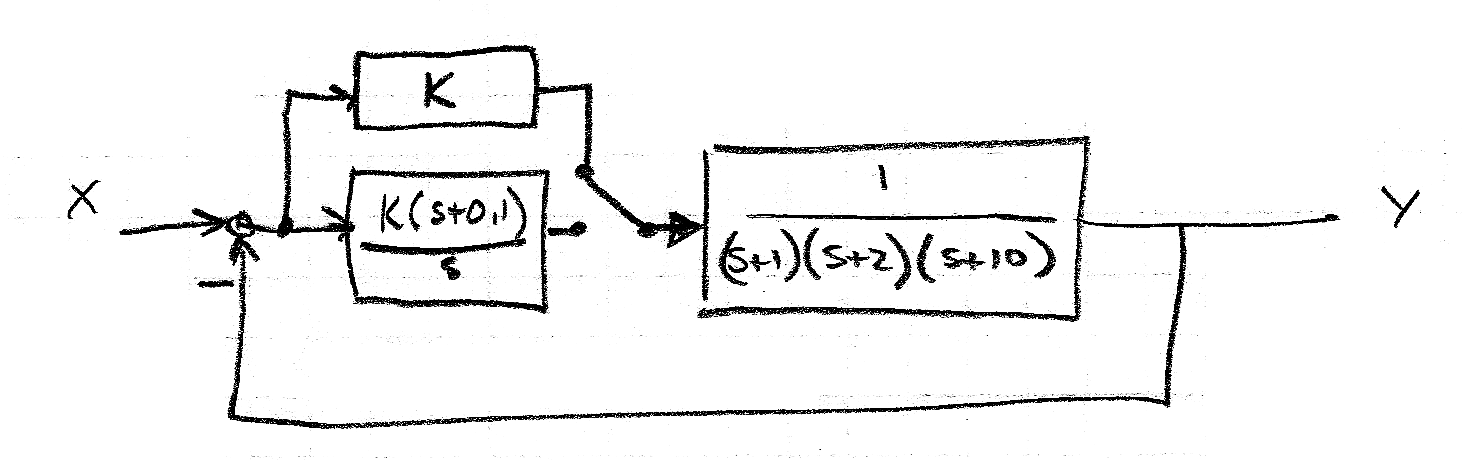
\includegraphics[width=100mm]{figs09/01107.png}

note that the PID version of these controllers is, 
\[
C_1(s):  \quad K_p = K \quad K_I = 0 \quad K_D = 0
\]
\[
C_2(s):  \quad K_p = K \quad K_I = 0.1K \quad K_D = 0
\]
Suppose we are asked  to find a type 1 controller with 
\[
T_s \leq 8sec \quad \%OS \leq 10\%
\]

Initially trying $C_1(s)$, draw the root locus and the performance lines:

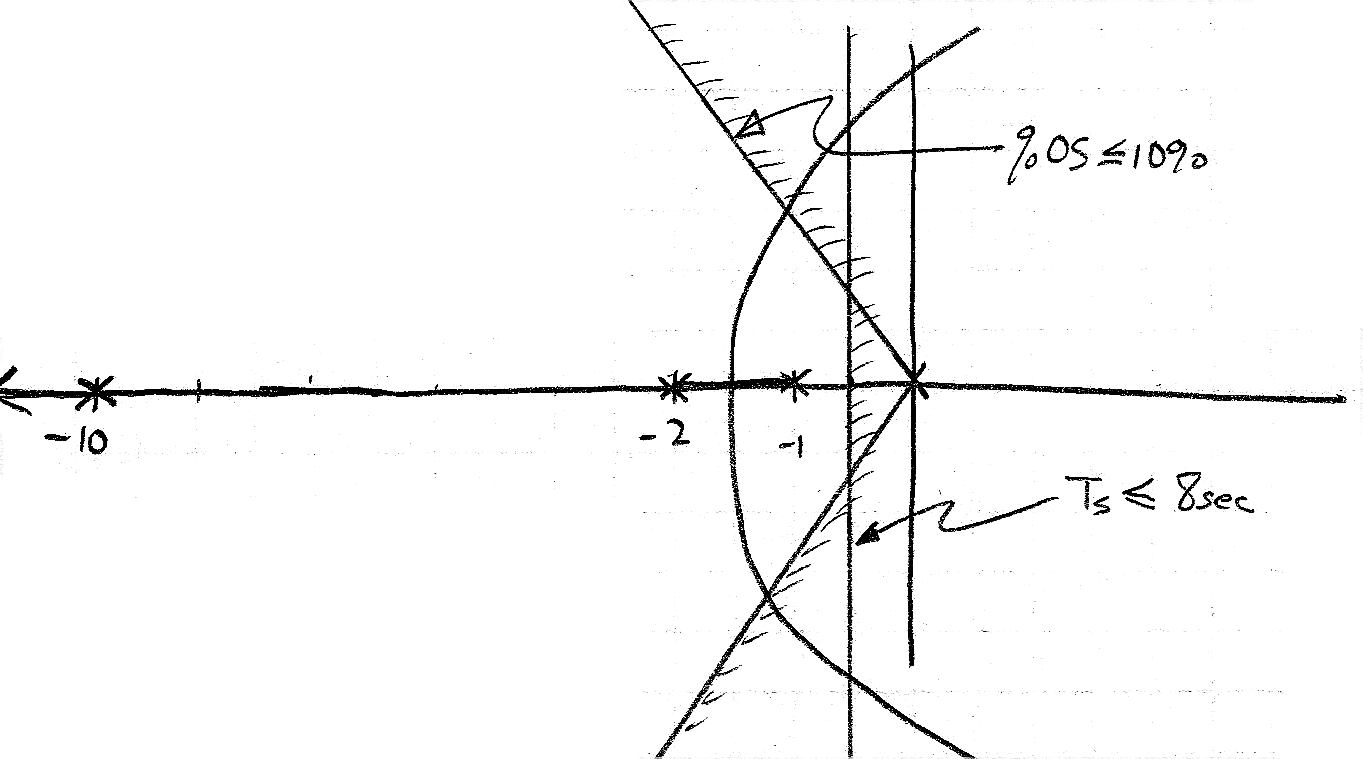
\includegraphics[width=100mm]{figs09/01108.png}

Although   there are clearly some values of $K$ which will satisfy the specs, the system is NOT type 1. 
To get type 1, we have to add a factor of $1/s$.  
\end{Example}
\begin{ExampleCont}
Now we consider the RL with $C_2(s)$.   First we sketch it without 
the performance regions for clarity.   

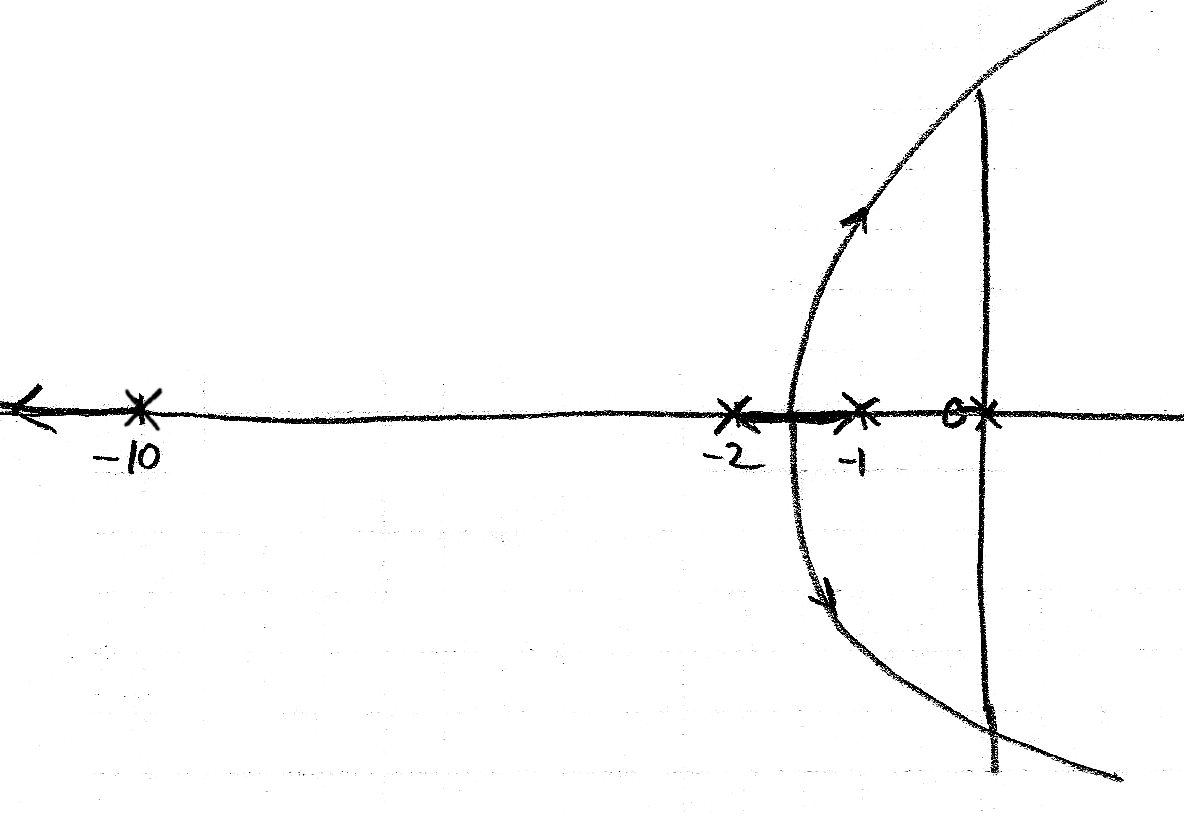
\includegraphics[width=85mm]{figs09/01109.png}

This root locus looks pretty close to what we had before.  
 $C_2(s)$ contains a pole ($s=0$) and zero ($s=-0.1$) which are close together relative to the plant poles.  Because
 of this they largely cancel their effects, but the system is still type 1(!).  Adding the performance regions: 
 
 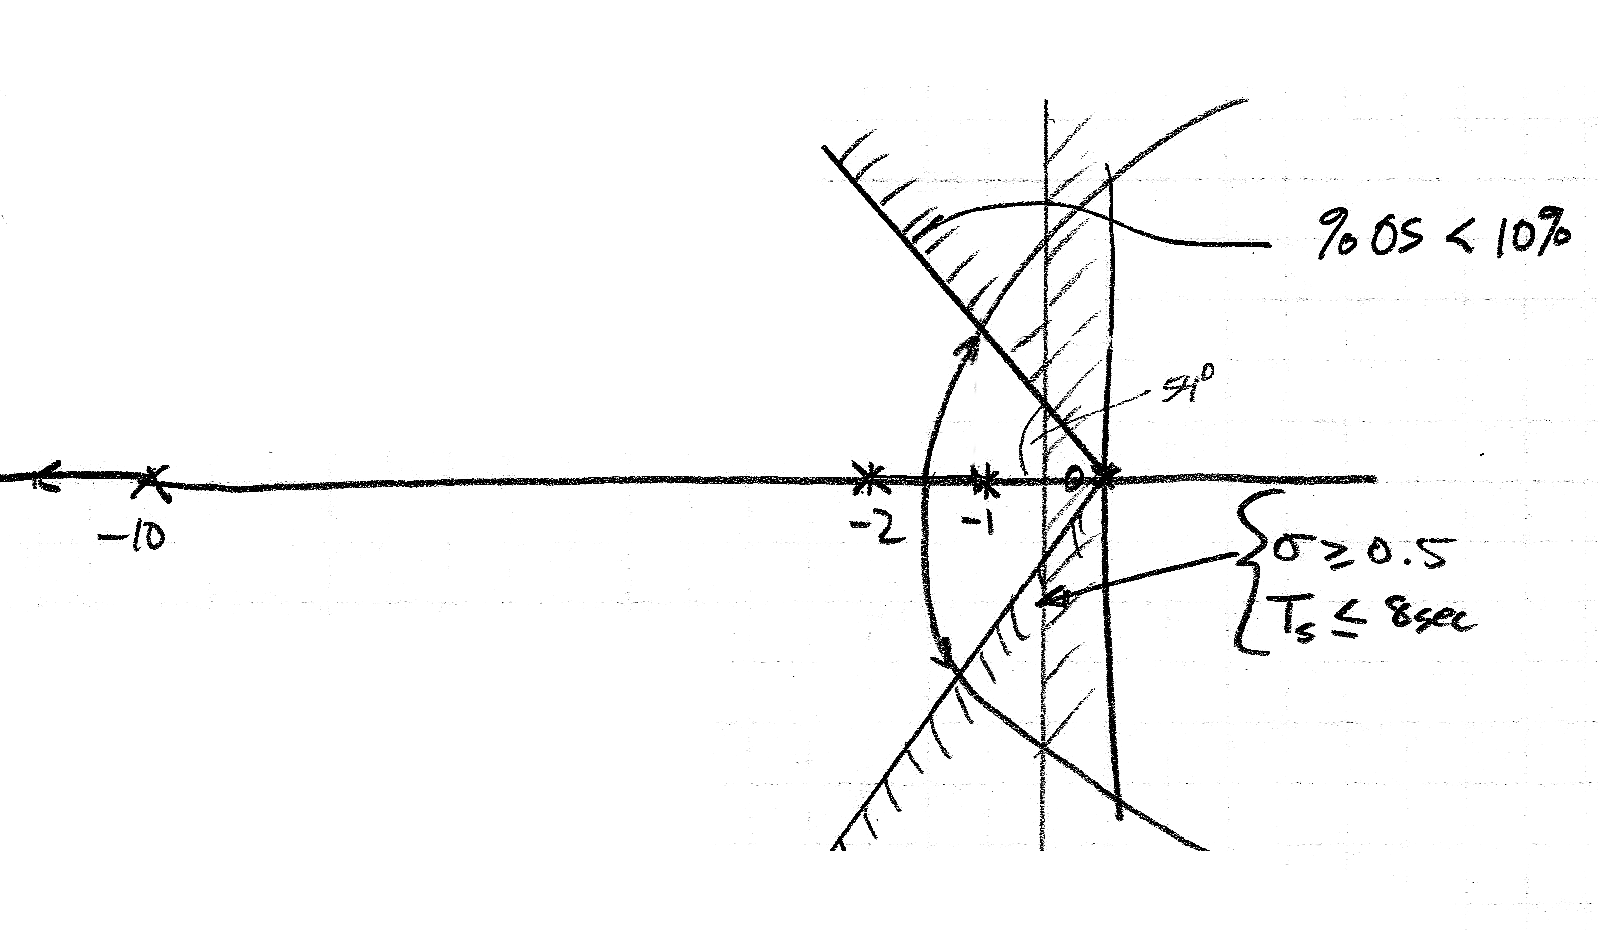
\includegraphics[width=110mm]{figs09/01110.png}

 We can now hand-compute $K$:
 
 \begin{enumerate}
   \item We will aim for the highest possible $K$ so we pick the point a little below where the RL crosses the diagonal \%OS line:
   about $s = -1.2+j1.2$.
   \item We know that all points on the RL satisfy the Magnitude Condition:
   \[
   |KCPH| = 1
   \]
   for our problem, $K$ is included in $C_2(s)$ and $H(s) =1$  so this is
   \[
   |C_2(s)||P(s)| = 1 \to  \frac   {K|-1.2+1.2j+1|} {|-1.2+1.2j|} = 1
   \]
   \item Solving for K:
   \[
   K = |0.2+1.2j|/|-1.2+1.2j| = 1.22/1.7 = 0.718
   \]
   
 \end{enumerate}
\end{ExampleCont}

%%%%** Example 12
\begin{Example}
We have a large industrial machine with the following plant model:

\[
P(s) = \frac {(s+1)} {(s+2.0)(s+0.7+0.2j)(s+0.7-0.2j)}, \quad H=1
\]


Our desired performance specifications are:

\[
T_{SD} = 1.33 sec  \qquad
\%OS = 10\%        \qquad
SSE_D = 0
\]
(Note that with these specs, there is a specific pole location rather than a region.)

It is decreed that we shall use a PID controller, but we have no initial values for $K_P, K_I, K_D$.

To approach the manual design, we will use the root locus method to analyze performance of PID controllers.  Because we need to plot zeros and poles of the controller,  the most useful form of the PID controller (for this design method) is:
\[
C(s) = \frac{K(s+z_1)(s+z_2)}{s}
\]
(we can convert this to $K_P, K_I, \mathrm{and} K_D$ using Equation \ref{PID2}.)

\subsubsection*{Problem Statement: }  Find values of $K, z_1, z_2$ (or equivalently $K_P, K_I, K_D$) that can be reasonably expected to meet the specifications.

\subsubsection*{Solution method}
\begin{enumerate}
 \item Make the assumption that the two complex conjugate plant poles closest to the origin are dominant (false!).
 \item Draw the s-plane and draw the region(s) corresponding to the performance specifications.


 \item Plot the poles and zeros of the plant on the s-plane.
 \item Place two zeros in places such that they will ``pull" the root locus through the target region\footnote{Assuming the plant poles do not already meet the specs(!)}.   

  \item Use Scilab to plot the Root Locus (``{\tt evans(sys)}" command)
  \item If the root locus goes through the target region, use the mouse to find the value of $K$ at the target location.
  \item Use the chosen $z_1, z_2$ and $K$ values to derive  $K_P, K_I, K_D$ (see Section \ref{Kpderive})
  \item If the root locus does NOT go through the target region, go back to step 4 and try again.
\end{enumerate}
% 
(continued next page)
\end{Example}
% 
% %%%%** Example 12
\begin{ExampleCont}

\subsubsection*{Method application}
The specifications are equality constraints (as opposed to inequalities) so the only point which satisfies both specs is the point where the vertical ($T_s$) and diagonal ($\%OS$) lines intersect.  For this problem that is the point $(-3 \pm j4.13)$.

In this example, we make an initial try of PID controller zeros at $s=-6\pm2j$ (step 4, above). 

The following hand drawn root locus explains why these {\it might} be good locations for the 
 zero.  

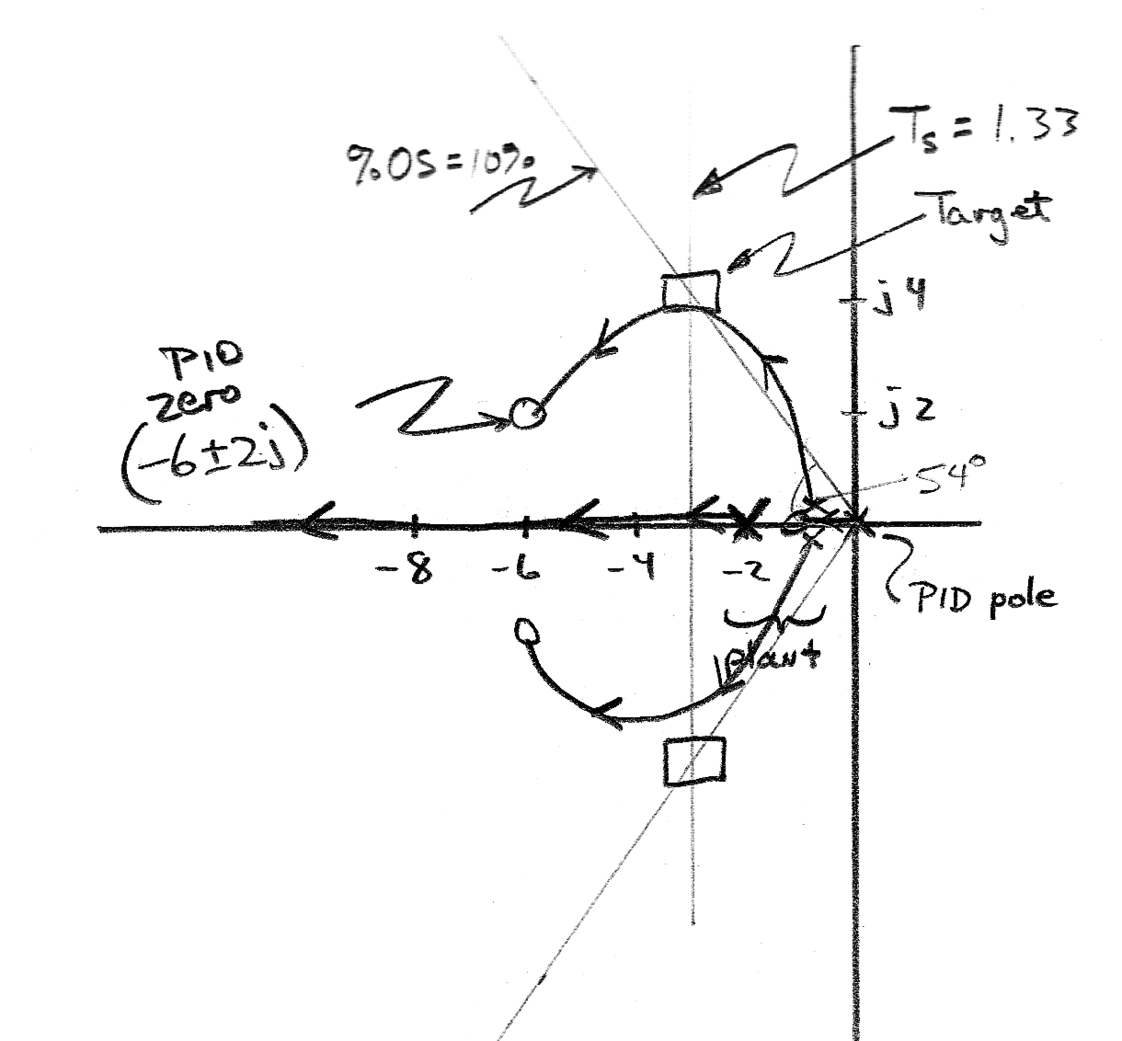
\includegraphics[width=95mm]{figs09/00823a.png}
 
However when we compute the root-locus using Scilab, it does not pass through the target.
  
Trying different zero locations in Scilab we find better results with two real 
zeros: $s= \{-1,-4\}$.

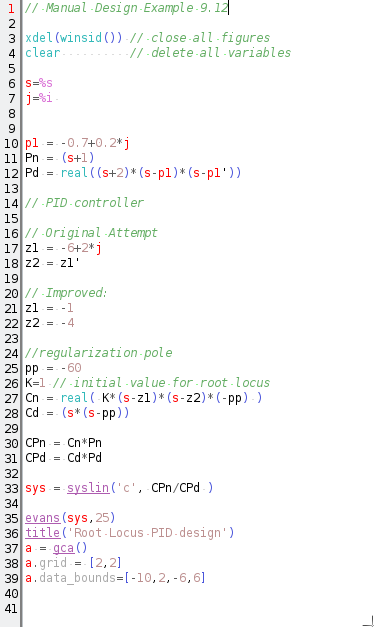
\includegraphics[width=62.5mm]{figs09/ex912ScilabCode.png}

\end{ExampleCont}
\begin{ExampleCont}
The computed Root Locus is

\begin{center}
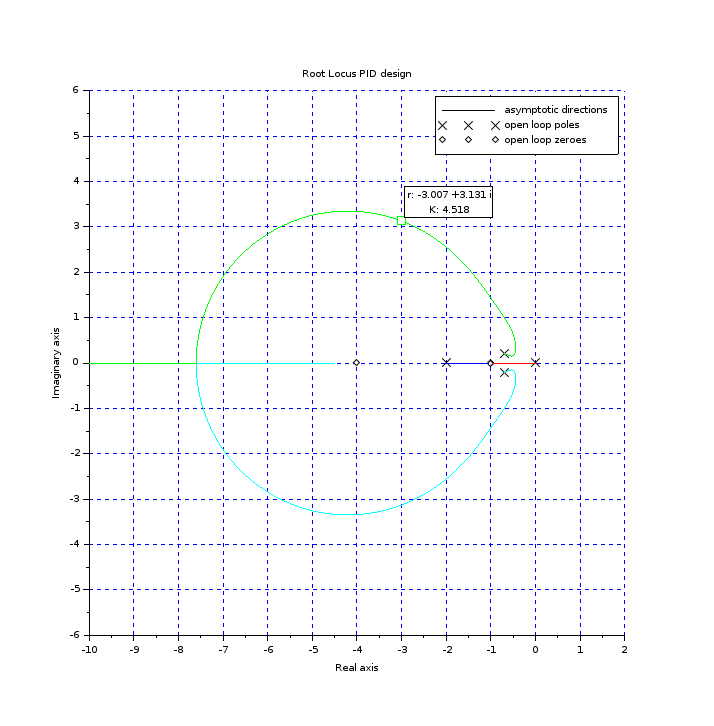
\includegraphics[width=115mm]{figs09/ex912RL.png}
\end{center}

 Note that now that at $s=-1$ we now have {\it two} zeros, one from 
the plant and one from the PID controler. 
Click on the small icon in upper left of the Root Locus graphics
window to enable ``Datatips" markers in the Scilab.   Then clicking on the root locus curve at or 
very near the target location, we find $K = K_D = 4.5$ (let's round it to 4.0 - this is only a rough
computation).

With $K_D$ and our PID zeros ($\{-1, -4\}$) known, we use Equation \ref{PID2} 
and the technique in Section \ref{Kpderive} (below) as follows:

\[
C(s) = \frac{4.0(s+1)(s+4)}{s} = \frac {4(s^2+5s+4)} {s}
\]
\[
= \frac{K_D}{s} \left ( s^2+\frac{K_P}{K_D}s + \frac{K_I}{K_D} \right )
\]

\[
K_P = 20 \qquad K_I = 16 \qquad K_D = 4
\]

\end{ExampleCont}

%%%%** Example 13
\begin{Example}
For the following system:
\[
P(s) = \frac {(s+3)} {s(s+1+1.5j)(s+1-1.5j)}  \qquad   H(s) = 1
\]
design a PID controller to achieve:
\[
T_S \leq 1.33 \qquad \%OS \leq 1\% \quad (34^\circ, \zeta = 0.83)
\]

Plotting the performance specs in the complex plane:

\begin{center}
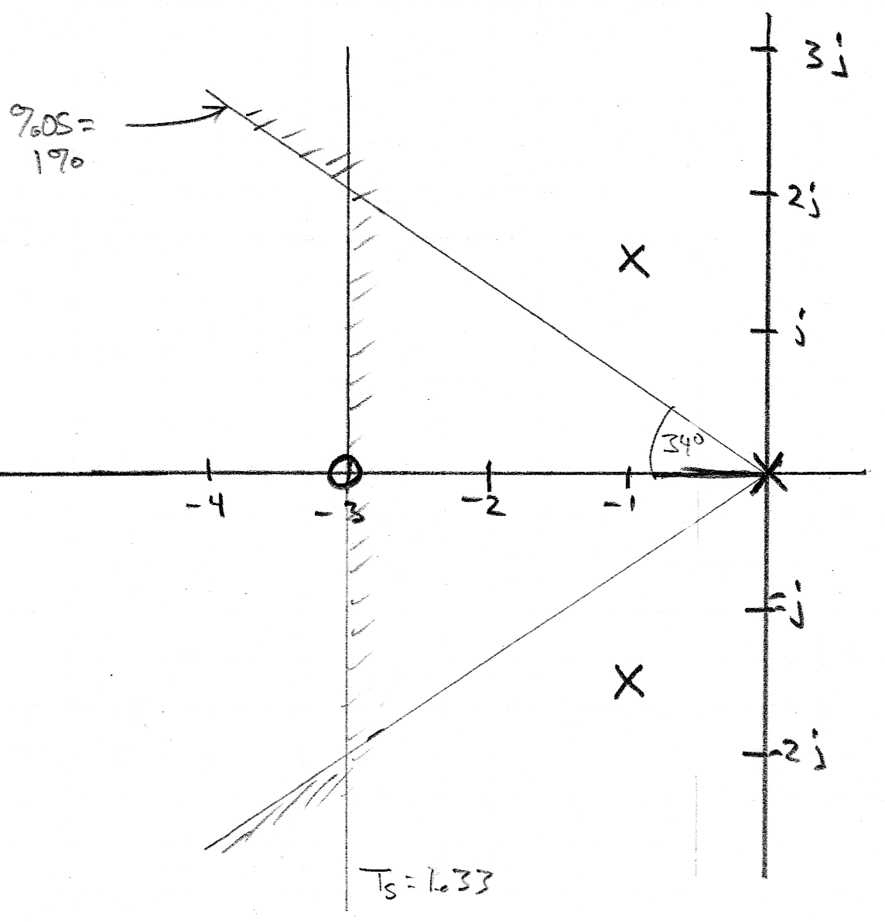
\includegraphics[width=75mm]{figs11/00928a.png}
\end{center}

The PID controller adds 2 zeros and a pole at the origin.   We hope that with some value of gain, it will move the closed loop poles to the left of the shaded region.

{\bf Try 1: } a double zero at $s=-1$ and a pole at the origin.   The resulting controller is
\[
C_1(s) = \frac{(s+1)(s+1)}{s}
\]
However, this cannot be simulated properly.   Using Section \ref{simulationPIDcontrollers}, we add a regularization pole at 20:

\[
C_1(s) = 20\frac{(s+1)(s+1)}{s(s+20)}
\]

Now we place this system into a Scilab script as follows:

\begin{verbatim}// EE447 PID Design Example (Design a PID Controller)
s=%s; j = %i;
//plant
p = (s+3)/(s*real((s+1+1.5*j)*(s+1-1.5*j)));
h = s/s;  // H=1 (you have to express in terms of s!)
pp = 20;  // regularization pole
// First guess controller
c1 = pp * ((s+1)*(s+1))/(s*(s+pp));
Sys = syslin('c', c1*p); //    loop gain system
clf();
evans(Sys,200);   // experiment with gain range (200)
a1=get("current_axes");          //get the handle of the newly created axesctl
a1.data_bounds=[-5,1, -3,3];
sgrid;  // helps for the % overshoot performance line
\end{verbatim}
\end{Example}

%%%%** Example 13
\begin{ExampleCont}
Running this script (and drawing some performance lines on the RL output) gives:

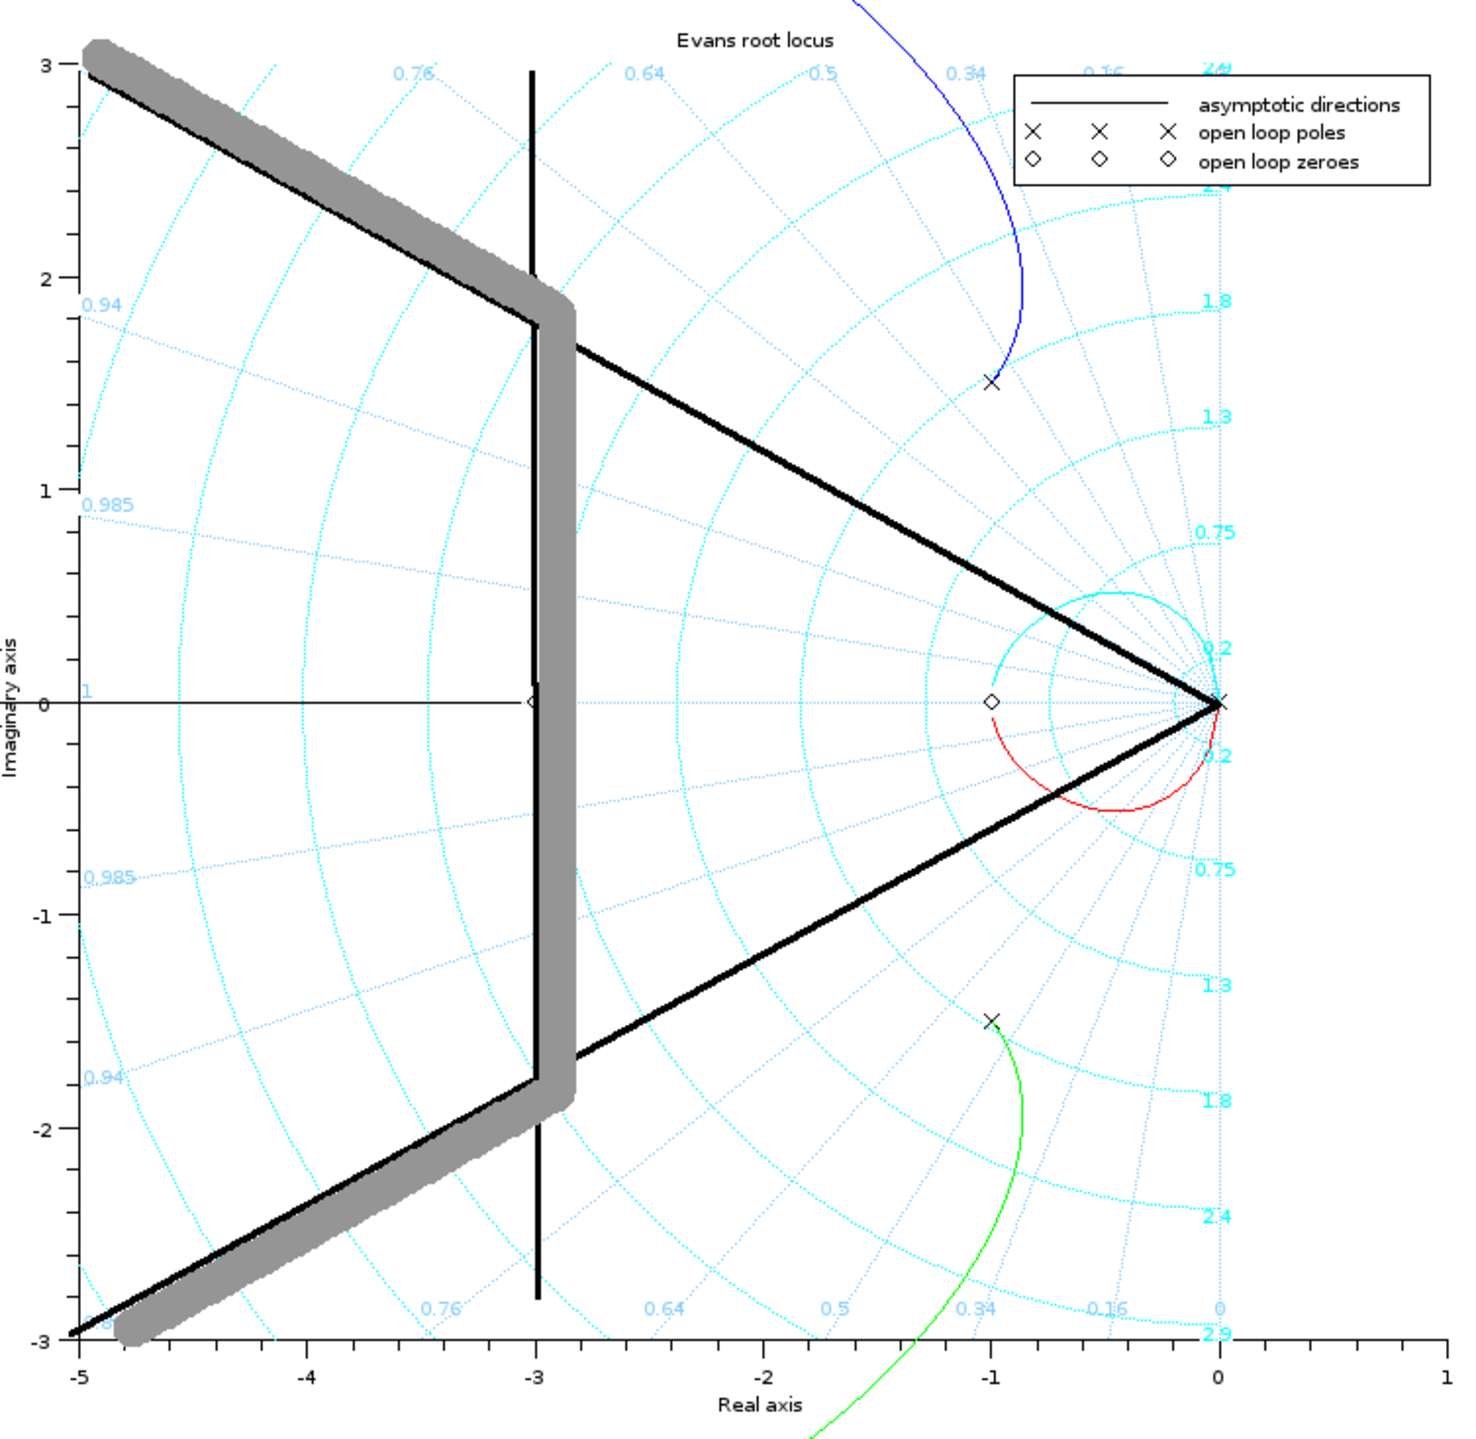
\includegraphics[width=125mm]{figs11/des_examp_01a.png}

Unfortunately, while some of the poles move into the region of acceptable performance\footnote{This can be seen with bigger values for {\tt a.data\_bounds}},
the two origin poles will never get to the left of $\sigma = -1$!

\vspace{0.2in}
{\bf Try 2: } Move the two zeros to $\{-5,-5\}$
\begin{verbatim}
// 2nd guess controller
pp=25;
c1 = pp * ((s+4)*(s+4))/(s*(s+pp));
Sys = syslin('c', c1*p); //    loop gain system
clf();
evans(Sys,2000);   // experiment with gain range (200)
a1=get("current_axes");          //get the handle of the newly created axesctl
a1.data_bounds=[-5,1, -3,3];
sgrid;  // helps for the % overshoot performance line
\end{verbatim}

\end{ExampleCont}

%%%%** Example 13
\begin{ExampleCont}
The resulting root locus is

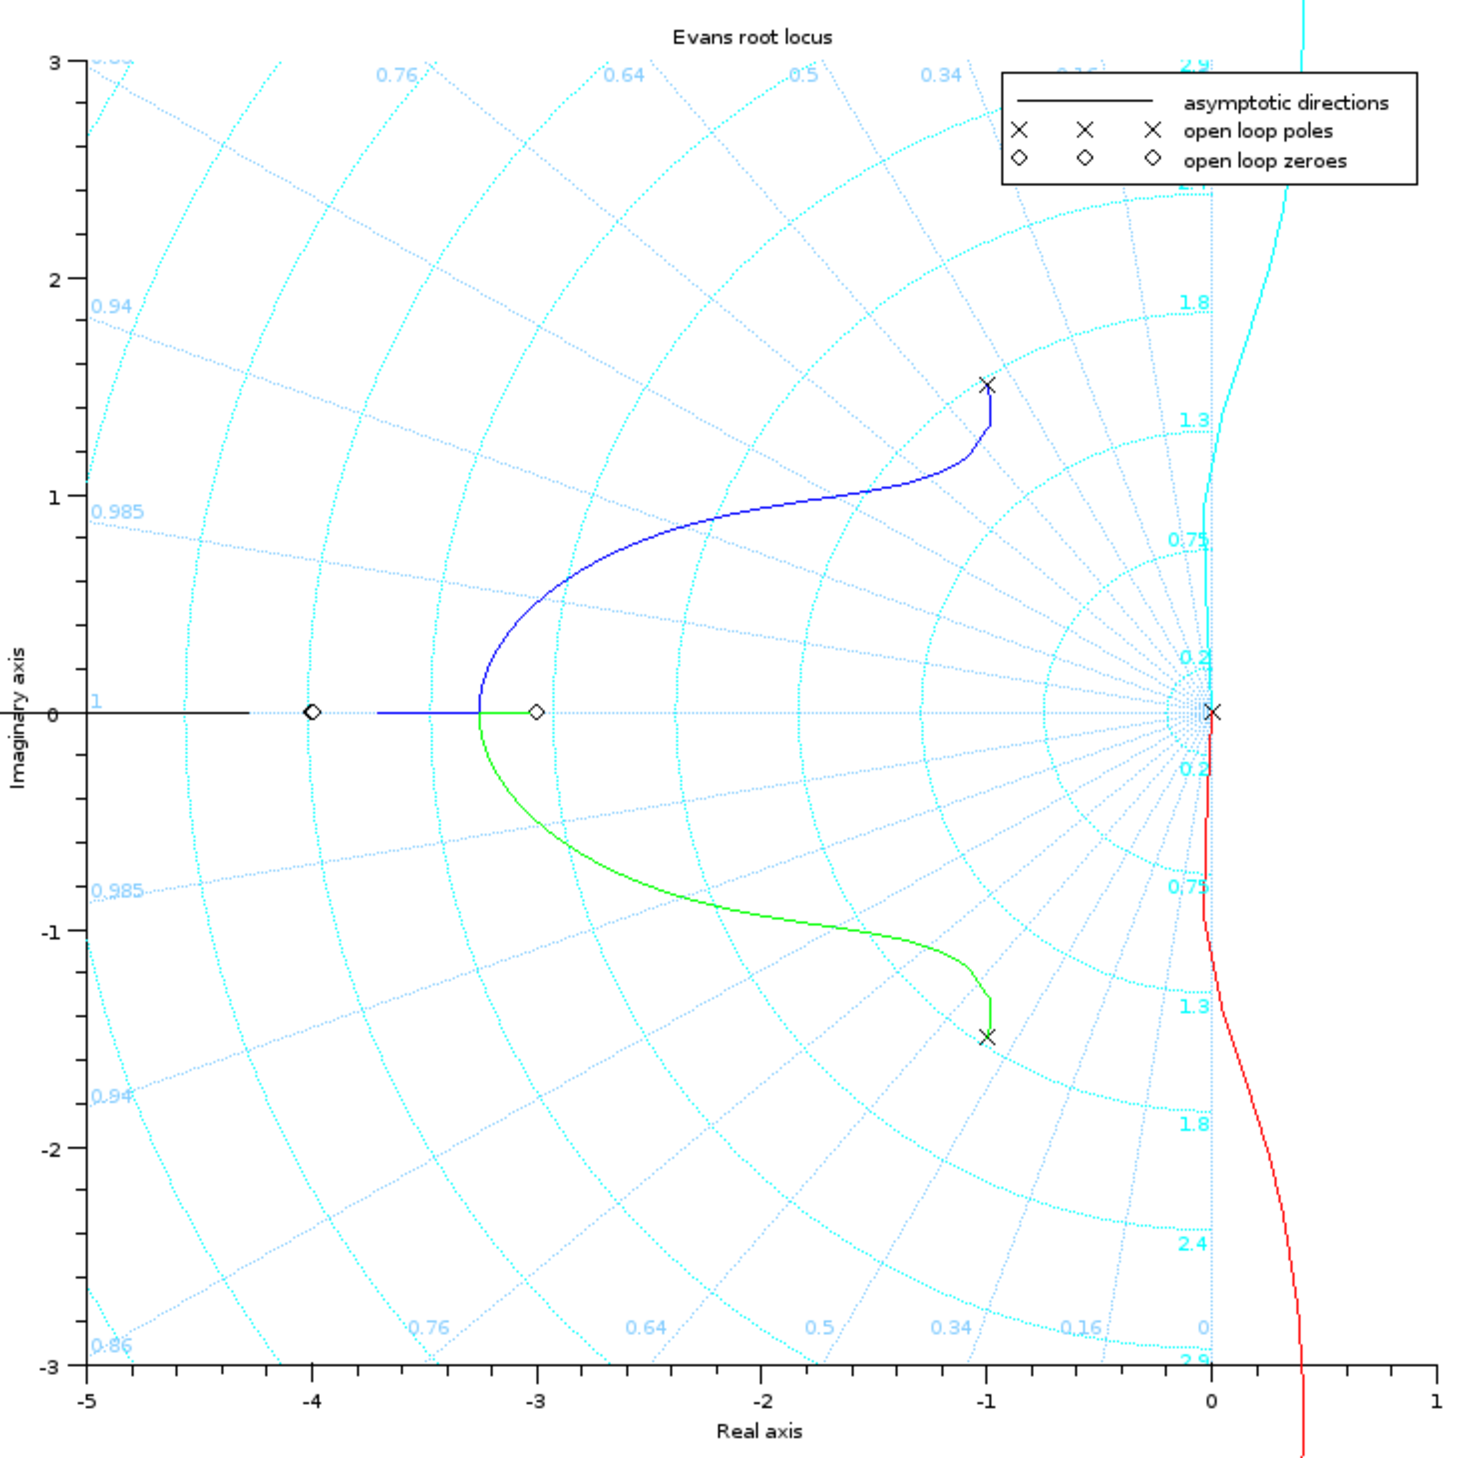
\includegraphics[width=125mm]{figs11/des_examp_02a.png}

There is no need to draw on the performance region because the two origin poles are now going unstable!  Very bad option.

Further root locus experimentation did not yield any controller which could be stable and have poles in the desired region!

What to do??    We must be sure to consider PID controllers where one of the paramters is zero.   Since we have a stability problem, we should take a hard look at adding a pole to the origin. 
The pole at $s=0$ is good for steady state error, but makes stability harder. 
We can eliminate this pole if we get rid of the integrator in the PID controller: $K_I = 0$ but this also eliminates one zero.  Using this ``PD" controller we have a zero and a gain as our remaining design parameters:
\[
C_{PD} = K(s+z) = K_Ds + K_P
\]

{\bf Try 3: }
\[
C_3(s) = K(s+0.1)
\]
\begin{verbatim}
// 3nd guess controller
c1 = pp*(s+0.1)/(s+pp);
Sys = syslin('c', c1*p); //    loop gain system
clf();
evans(Sys);   // experiment with gain range (200)
a1=get("current_axes");          //get the handle of the newly created axesctl
a1.data_bounds=[-5,1, -3,3];
sgrid;  // helps for the % overshoot performance line
\end{verbatim}


\end{ExampleCont}

%%%%** Example 13
\begin{ExampleCont}
The root locus is now:

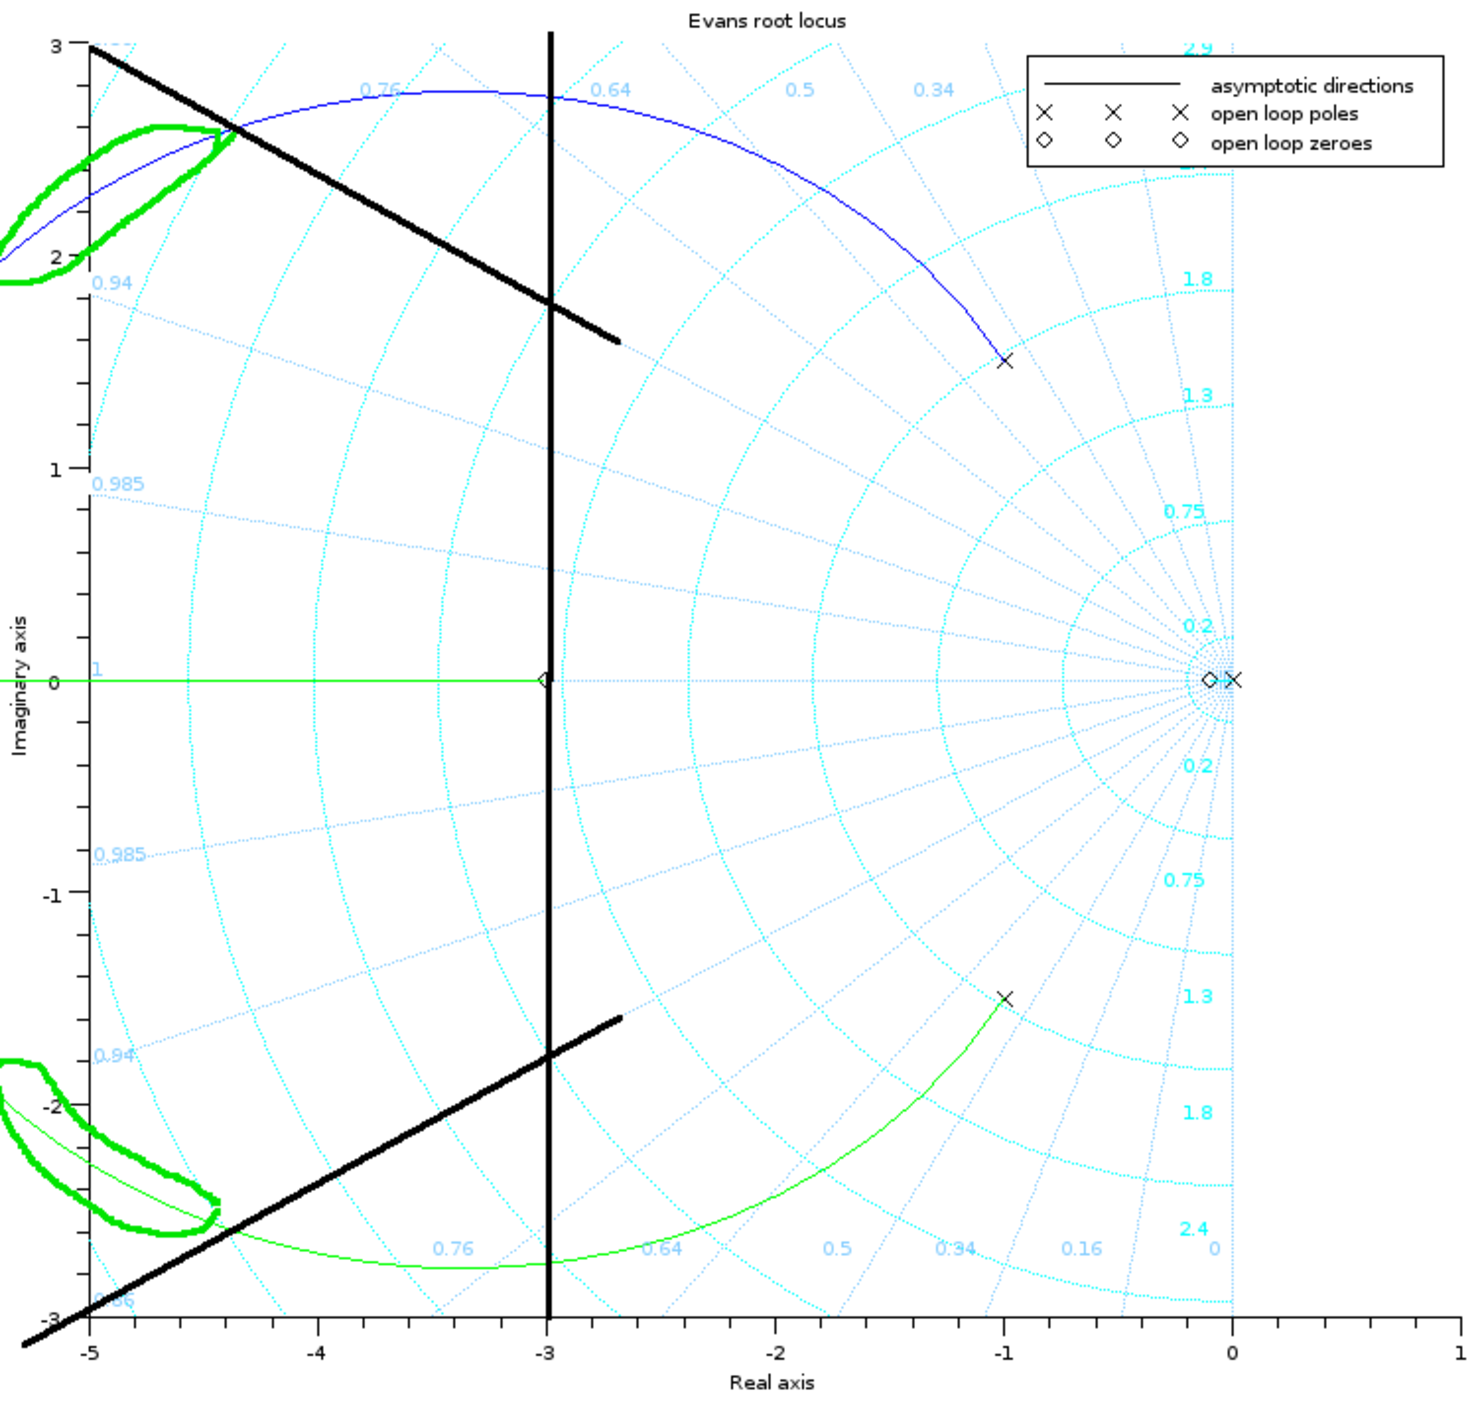
\includegraphics[width=125mm]{figs11/des_examp_03aa.png}

which allows the poles to move into the zone (green circled parts of RL).   Using the mouse to click on the part of the RL indicated gives $5.6 < K < 6.4$.  Using K=6.0,
\[
K_P = 0.6, K_I = 0.0,  K_D = 6.0
\]

You might notice that the pole at the origin moves only slightly and arrives at the 
PD controller zero we placed at $\sigma=-1$.  This one does not lie in the performance 
region.  One way to look at this is that the pole and zero being very close to each other 
``cancel each other out" in the closed loop response.   
This exposes a limitation of the ``$T_s, \%OS$ / s-plane region" approach to control 
design, which is that the regions are only truely valid with a pure second order system 
with two poles and no zeros.  For all other systems the regions are really only approximate. 

At this point we have reached a good starting point for computer optimization which 
will NOT make simplifying assumptions about the system dynamics or performance regions. 
\end{ExampleCont}



%%%%** Section 5.1
\subsection{Deriving $K_P, K_I, K_D$ from controller zeros}\label{Kpderive}

There are several forms of the PID controller including:
\[
C(s) = K_D \left ( s^2+ \frac{K_P}{K_D}s + \frac{K_I}{K_D} \right ) \frac{1}{s}
\]
Let
\[
PC(s) = \left ( s^2+ \frac{K_P}{K_D}s + \frac{K_I}{K_D} \right )
\].

Suppose that zero locations we like are
\[
z_i = (s + 1.7 \pm 0.5j)
\]
and that the result of step 5 above yields $K_D = 1.85$.   Multiplying out gives
\[
PC(s) = (s + 1.7 + 0.5j)(s + 1.7 - 0.5j)  = s^2 + 3.4s + 3.14
\]
Therefore,
\[
C(s) = 1.85 PC(s) \frac{1}{s} = 1.85(s^2 + 3.4s + 3.14)\frac{1}{s}
\]
\[
C(s) = 1.85s + 6.29 + \frac {5.809} {s} = 6.29 + \frac {5.809} {s} + 1.85s
\]
Giving us
\[
K_P = 3.4\times 1.85 = 6.29   \qquad  K_I = 3.14\times1.85 = 5.809 \qquad K_D = 1.85
\]
This gives us a rough design to start the computer optimization process.



% \section{Summary of Notation}

